%XXX: Aaron, do one last check for new typos in my final series of edits.
\documentclass[preprint,11pt]{aastex} 
\let\captionbox=\undefined
\usepackage[top=1in, bottom=1in, left=1in, right=1in]{geometry}
\usepackage{amsmath}
\usepackage{graphicx}
\usepackage{mdwlist}
\usepackage{natbib}
\usepackage{natbibspacing}
\usepackage[font={footnotesize}]{caption}
\usepackage{wrapfig}
\usepackage{sidecap}
\usepackage{tabularx}
\usepackage{enumitem}
\usepackage{url}
\setlist[itemize]{noitemsep, topsep=0pt}
\setlist[enumerate]{noitemsep, topsep=0pt}
\setlength{\bibspacing}{0pt}
\setlength{\parskip}{0pt}
\setlength{\parsep}{0pt}
\setlength{\headsep}{0pt}  
\setlength{\topskip}{0pt}
\setlength{\topmargin}{0pt}
\setlength{\topsep}{6pt}
\setlength{\partopsep}{0pt}
\setlength{\footnotesep}{8pt}
\pagestyle{plain}
\citestyle{aa}
\captionsetup[table]{labelsep=space}
\captionsetup[figure]{labelsep=space}

%%% ADDED FROM 2014 PROPOSAL
%\newcommand{\Mycite}[1]{{\bf \cite{#1}}}
%\newcommand{\Mycitet}[1]{{\bf \citet{#1}}}
%\newcommand{\Mycitep}[1]{{\bf \citep{#1}}}
%\newcommand{\Mycitealt}[1]{{\bf \citealt{#1}}}
\newcommand{\Mycite}[1]{\cite{#1}}
\newcommand{\Mycitet}[1]{\citet{#1}}
\newcommand{\Mycitep}[1]{\citep{#1}}
\newcommand{\Mycitealt}[1]{\citealt{#1}}

\newcommand{\kvec}{{\bf k}}
\newcommand{\bvec}{{\bf b}}
\newcommand{\shat}{{\hat s}}
\newcommand{\kpr}{{k_\perp}}
\newcommand{\kvpr}{{\kvec_\perp}}
\newcommand{\AI}{{\langle\tilde A*\tilde I\rangle}}
\newcommand{\AItau}{{\AI(\tau)}}
\newcommand{\hMpci}{{h~{\rm Mpc}^{-1}}}
\newcommand{\inch}{$^{\prime\prime}$}
\newcommand{\foot}{$^{\prime}$}
\renewcommand{\deg}{^\circ}

\newcommand{\simgt}{\stackrel{>}{_{\sim}}}
\newcommand{\compress}{\vspace{-0.25in}}
\newcommand{\captionbaseline}{\renewcommand{\baselinestretch}{0.99}} 
\newcommand{\Caption}[4]{\vspace{#1}\renewcommand{\baselinestretch}{#2}\caption{#4}\vspace{#3}}
\def\kperp{k_{\bot}}
\def\eppsilon{{$\varepsilon$ppsilon}}
\def\kpar{k_{\|}}
\def\k{{\bf k}}
\def\sky{{\theta}}
\def\HI{{H{\small I }}}
\def\HII{{H{\small II }}}
\def\xHI{{x_{\rm\HI}}}
\newcommand{\startsquarepar}{%
    \par\begingroup \parfillskip 0pt \relax}
\newcommand{\stopsquarepar}{%
    \par\endgroup}

%%% UNCOMMENTED
\usepackage{subfig}
%\usepackage[countmax]{subfloat}
\title{Hydrogen Epoch of Reionization Array (HERA)}
\author{A.U.Thor}

\begin{document}
\maketitle

\begin{center}
\textbf{Abstract}
\end{center}

The Hydrogen Epoch of Reionization Array (HERA http://reionization.org) is a staged experiment that uses the unique properties of the 21-cm line from neutral hydrogen to probe the Epoch of Reionization (EOR). During this epoch, roughly 0.3 - 1 billion years after the Big Bang, the first galaxies and black holes heated and reionized the early Universe. Direct observation of the large scale structure of reionization and its evolution with time will have a profound impact on our understanding of the birth of the first galaxies and black holes, their influence on the intergalactic medium (IGM), and cosmology.  This paper will provide an overview of the project and describe the design of the system.

\section{Introduction}

\noindent The Hydrogen Epoch of Reionization Array (HERA) is a staged experiment to use the redshifted 21\,cm line
of neutral hydrogen to characterize our Cosmic Dawn, from
the formation of the first stars and black holes $\sim0.1~$Gyr after the Big
Bang ($z\sim30$) through the full reionization of the intergalactic medium
(IGM) $\sim1~$Gyr later ($z\sim6$).  By directly observing the large scale
structure of the primordial IGM as it is heated and reionized, HERA complements
other probes, adding transformative capabilities for
understanding the astrophysics and fundamental cosmology of our early universe.
Taking advantage of our new mastery of bright foreground systematics, HERA's
purpose-built radio
interferometer is optimized to deliver high signal-to-noise measurements of
redshifted 21\,cm emission.
With the first generation 21\,cm telescopes approaching the limits of their sensitivity, HERA continues the experiment by bringing significantly more sensitivity to bear
while continuing to optimize its design along the delay-spectrum approach.

\begin{figure}[h!]
	\centering
	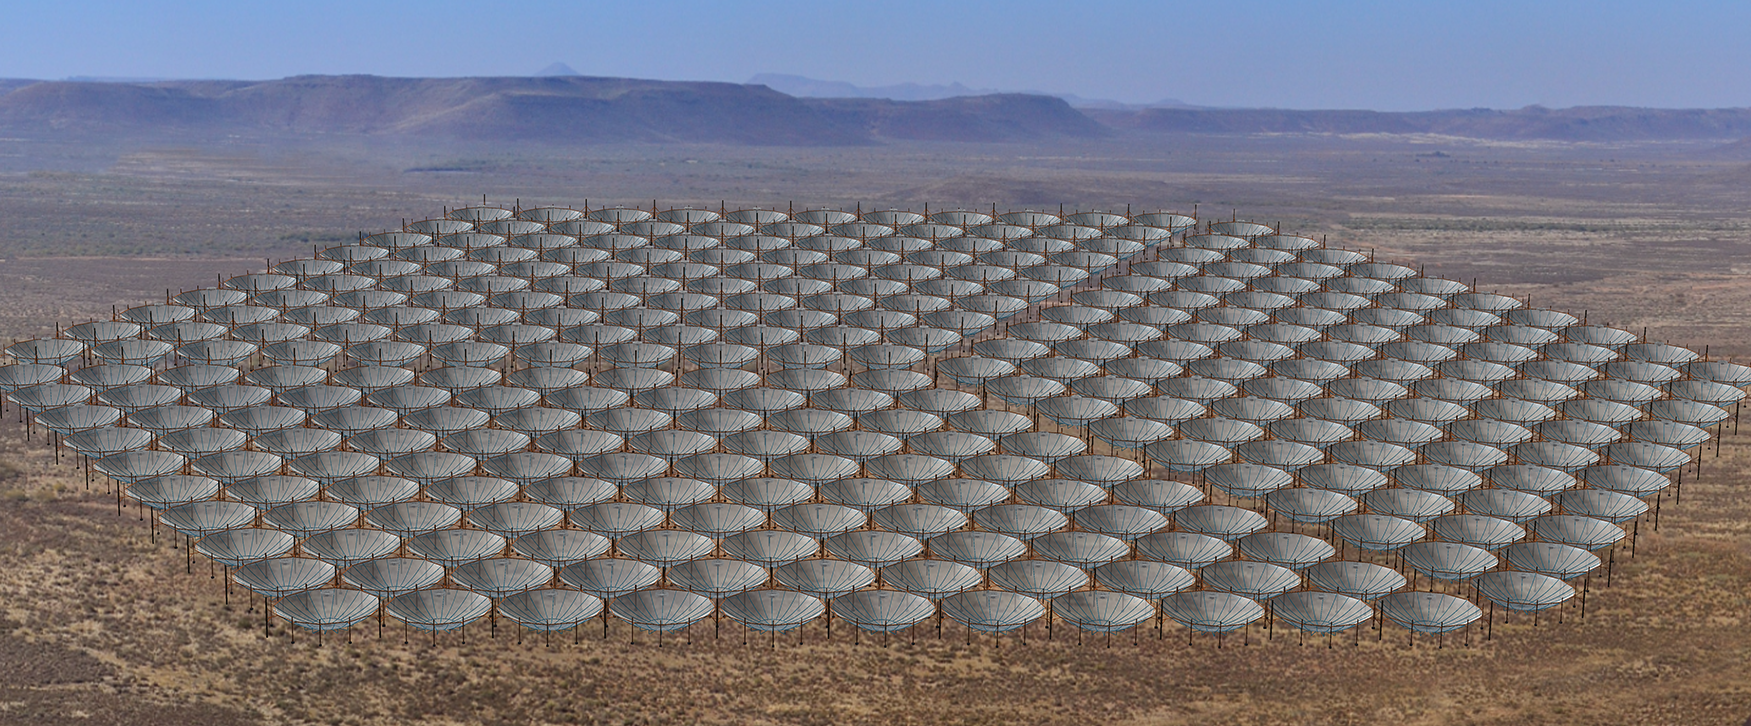
\includegraphics[height=1.75in]{plots/hera_render.png}
	\includegraphics[height=1.75in]{plots/hera19H.png}
	\caption{Rendering of the 320-element core (left) of the full HERA-350 array and picture of 19 HERA 14-m, zenith-pointing dishes (with PAPER elements in the background) currently deployed in South Africa (right).} 
	\label{fig:HERApictures}
\end{figure}

HERA brings to bear both the sensitivity and the precision to deliver 
its key science results on the basis of proven techniques.
These science results include
\begin{itemize}[noitemsep,nolistsep]
\item measuring the 21\,cm power spectrum with high significance (\S\ref{sec:EoRPowerSpectra}),
\item characterizing parametrized models of reionization and the first ionizing sources (\S\ref{sec:EoRPowerSpectra}),
\item improving cosmic microwave background (CMB) constraints on primordial density fluctuations and neutrino masses by removing the optical depth degeneracy (\S\ref{sec:tau}), and
\item directly imaging large scale reionization structure (\S\ref{sec:imaging}).
\end{itemize}
At the same time, HERA continues the development of new techniques that extend and improve its capabilities.
Examples include improving foreground subtraction to expand the information content 
in power spectral and imaging measurements and, with support from the Moore Foundation,
extending HERA's performance at lower frequencies to probe IGM heating in the pre-reionization epoch (\S\ref{sec:EoX}).
Beyond these directly supported applications, HERA's public data products and instrumentation platform enable other high-impact science, including 
\begin{itemize}[noitemsep,nolistsep]
\item 21\,cm cross-correlation (e.g. with JWST, WFIRST, CO, CII, and Ly$-\alpha$; \S\ref{sec:crossCorr}),
\item searching for auroral radio bursts from exoplanetary magnetospheres (\S\ref{sec:exoplanets}), and
\item performing triggered, low-frequency follow up and characterization of fast radio bursts (\S\ref{sec:FRBs}).
\end{itemize}

The HERA experiment will comprise 
350 14-m parabolic dishes (320 in a dense core $+$ 30 outriggers) in the South African Karoo Radio
Astronomy Reserve.
HERA has been funded under the US National Science Foundation's Mid-Scale Innovations Program to begin building elements optimized for robust power spectrum detection in a 
staged deployment.  The key is to produce inexpensive collecting area optimized to detect the EOR.  This has resulted in a close-packed array of transit 14-meter dishes (Fig. \ref{fig:HERApictures}), with the first 19-element array completed and construction underway for 37 elements, when the first science observing will begin.
The first phase, extending to August 2016, will deploy 37 elements that will test the HERA element design for performance and manufacturability at location.  These 37 elements will more 
than double the sensitivity of the 128-element PAPER array.  The next proposed phase will build out to 128 elements and use the existing 128 dual-polarization analog and digital signal 
paths along with , which should provide a very robust detection of the EOR signal.  Finally, extending into 2020, HERA will build out to 350 elements to further EOR science as a function 
of redshift and spatial scale, potentially producing the first images of the EOR.

HERA is a collaboration of the following Partner institutions:  
Arizona State University (Tempe, AZ USA), 
Brown University (Providence, RI USA), 
University of California Berkeley (Berkeley, CA USA), 
University of California Los Angeles (Los Angeles, CA USA), 
University of Cambridge (Cambridge, UK), 
Massachusetts Institute of Technology (Cambridge, MA USA), 
National Radio Astronomy Observatory (Charlottesville, VA USA), 
University of Pennsylvania (Philadelphia, PA USA), 
Scuola Normale Superiore di Pisa (Pisa, Italy),
SKA-South Africa (Cape Town, South Africa), and
University of Washington (Seattle, WA USA).  
Additional Collaborators are at 
Harvard University (Cambridge, MA USA),  
University of KwaZulu Natal (Durban, South Africa), 
University of Western Cape (Cape Town, South Africa), 
Imperial College London  (London, UK) and 
California State Polytechnic University (Pomona, CA USA).

This paper has the following structure.  Section \ref{sec:science} will give a high-level overview of the science motivating HERA's construction, including primary and secondary science objectives.  Section \ref{sec:eormeas} will present the techniques used to make the measurement, focussing on the delay-spectrum approach.  Section \ref{sec:requirements} will present the resulting high-level requirements and section will present the system description \ref{sec:design} as the bulk of the paper.   Section \ref{sec:status} will provide a status and section \ref{sec:conclusion} will conclude by summarizing and providing additional context.

\section{Scientific Background}
\label{sec:science}

\noindent The {\it Cosmic Dawn} of our universe is one of the last unexplored
frontiers in cosmic history, which is summarized in the cartoon in Fig. \ref{fig:cosmos}. During this period, the 
intergalactic medium (IGM) encodes a panoply of information about astrophysical and cosmological phenomena. 
This period saw the evolution of the universe from a very homogeneous ``gas'' to the formation of the first stars and galaxies.
Ultimately this early population of gravitationally condensed material produced sufficiently energetic flux to reionize the IGM
from its previous neutral state in a period called the Epoch of Reionization
Its evolution depends on the cosmic density field, the relative velocities of
baryons and dark matter, and the sizes and clustering of the first galaxies.
But it also depends on the constituents of those galaxies---so-called Population
III stars (stars formed very early with little to no elements heavier than helium), later generation stars, stellar remnants, X-ray binaries,
and early supermassive black holes.  Bulk properties like
ultraviolet and X-ray luminosities and spectra also affect the thermal and
ionization states of the IGM.  The wealth of unexplored physics during the Cosmic Dawn,
culminating in the Epoch of Reionization, 
led the most recent US National Academies astronomy decadal survey entitled {\em New Worlds, New Horizons} (NWNH) to highlight it as one of the top three ``priority science objectives'' for
the decade.

\begin{figure}[h!]
	\centering
	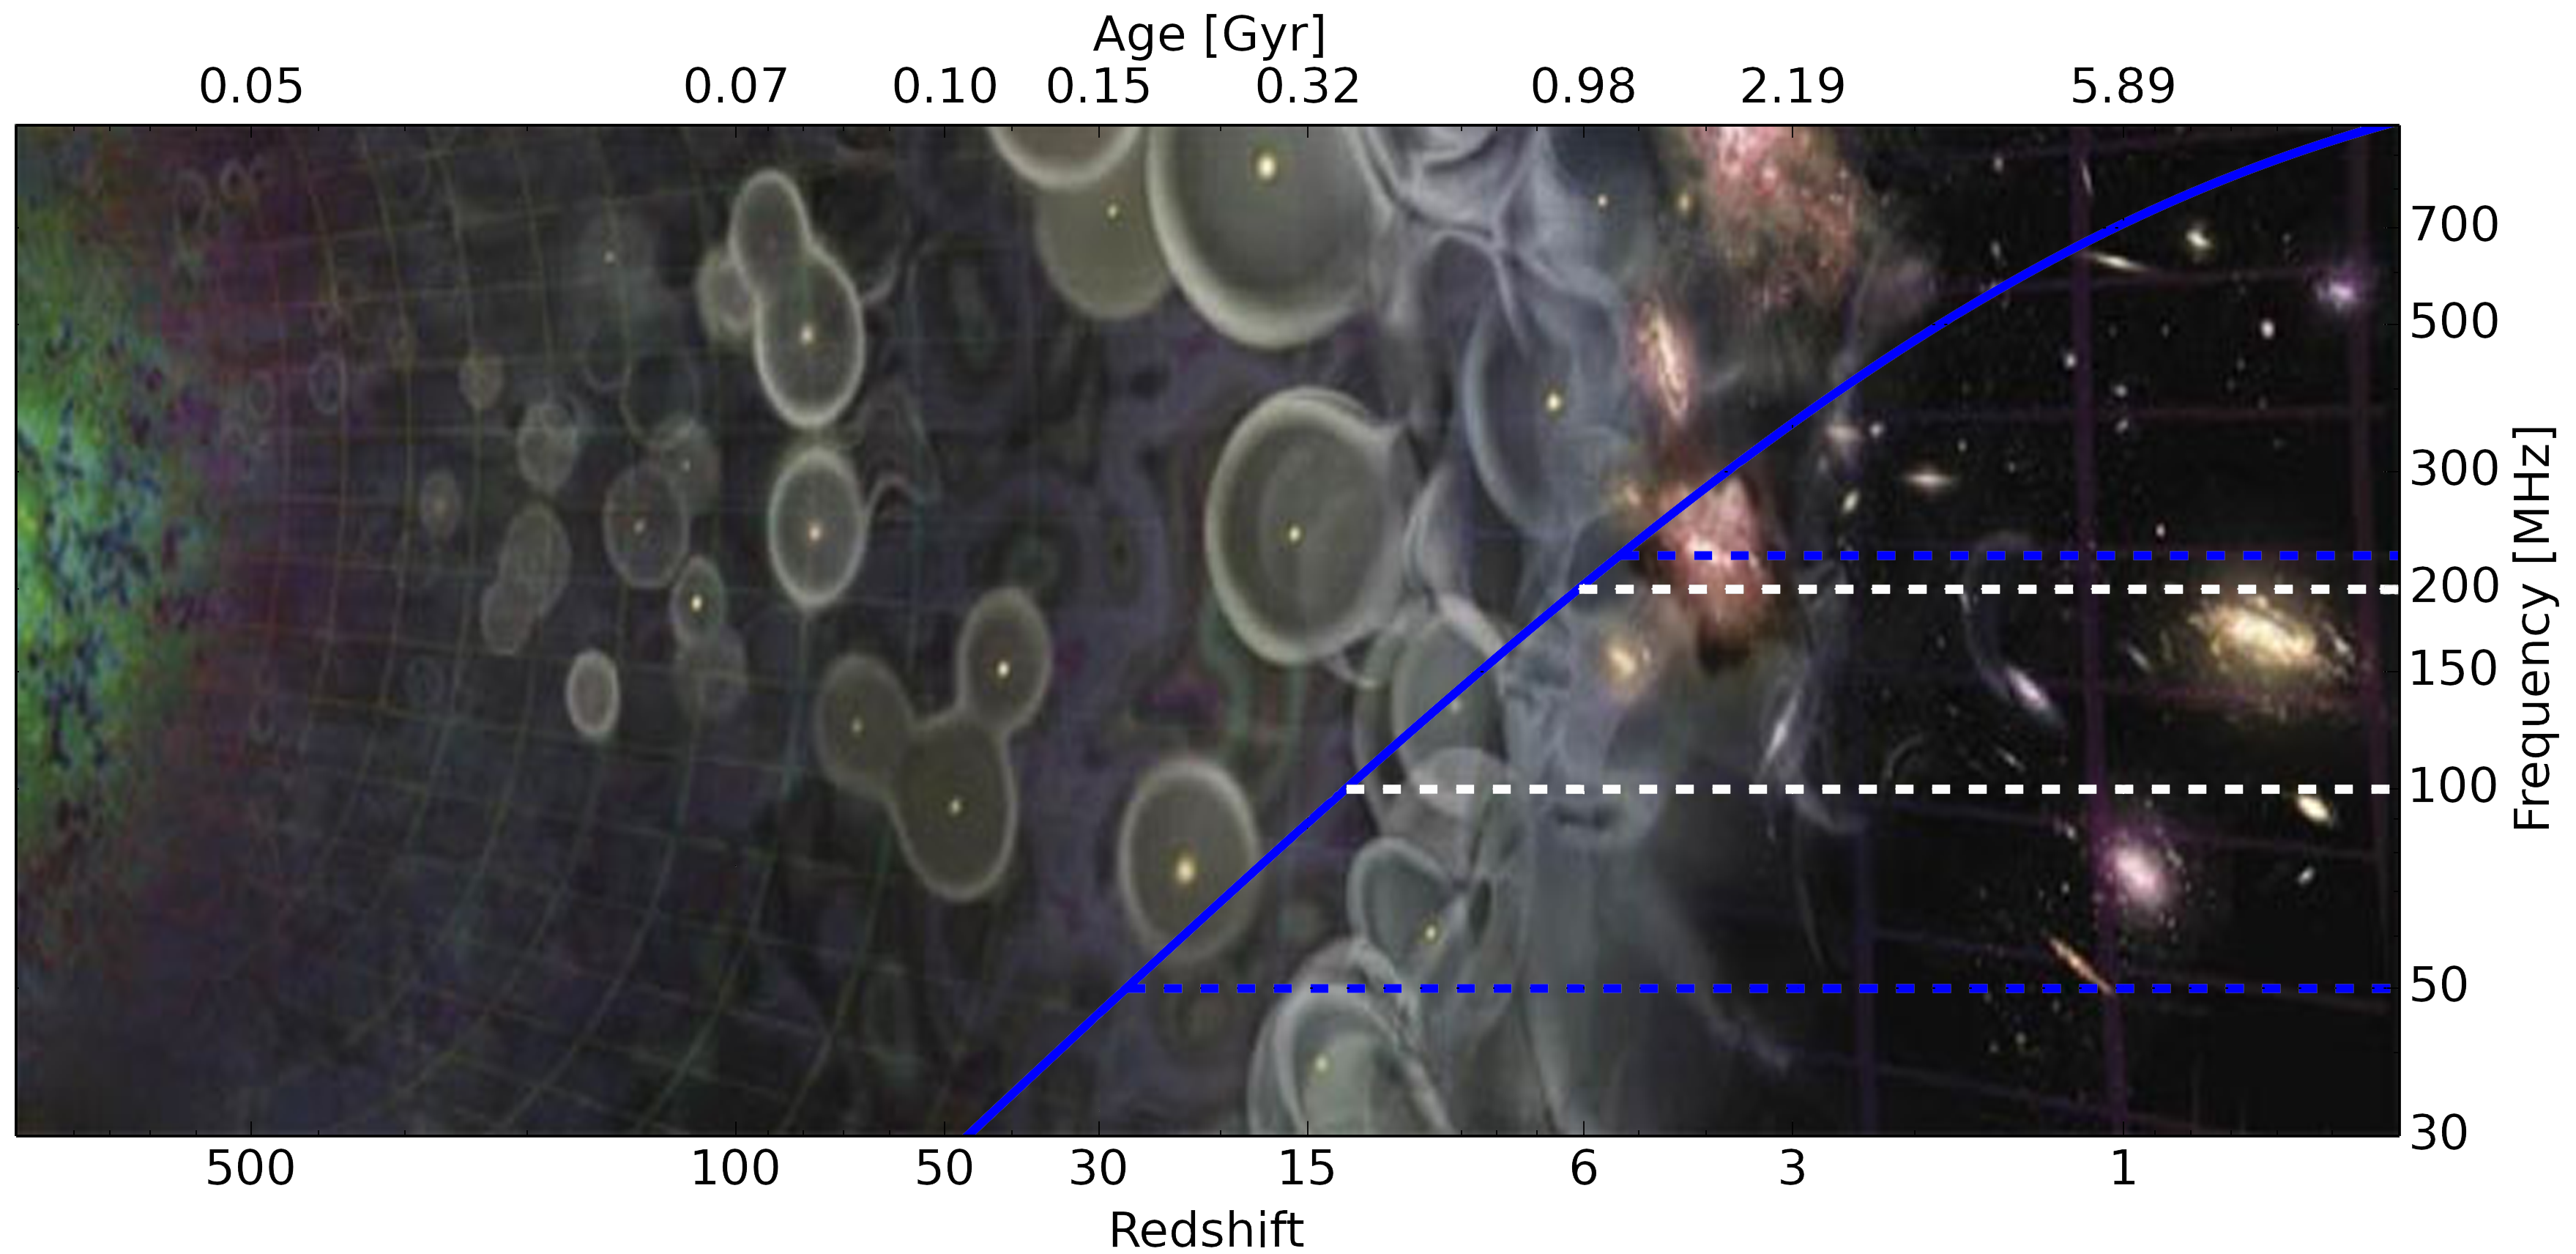
\includegraphics[width=0.7\textwidth]{plots/cosmicEvo.png}
	\caption{Rendering of cosmic evolution from just after the Big Bang to today (credit CCCCC).  The blue line shows the frequency of the red-shifted hydrogen line (rest frequency 1420 MHz) as a function of redshift (lower horizontal axis) and cosmic time (upper horizontal axis).} 
	\label{fig:cosmos}
\end{figure}


Exploring the interplay of galaxies and large-scale structure during the EOR
requires complementary observational approaches. CMB measurements 
provide initial conditions for structure formation, and the Thomson
scattering of CMB photons constrains the integrated column of 
ionized gas, but even with kinetic Sunyaev-Zel'dovich measurements, 
the detailed evolution of the IGM 
is only loosely constrained \citep{haiman_holder2003,mortonson_hu2008,mesinger_et_al2012}.
Lyman-$\alpha$ absorption features in quasar and $\gamma$-ray burst spectra give 
ionization constraints at the tail end of reionization 
($z\la7$, \citealt{fan_et_al2006, mcgreer_et_al2015}), but these features 
saturate at low neutral fractions
($x_{\rm HI} \la 10^{-4}$). Measurements of galaxy populations in
deep {\it Hubble Space Telescope} observations 
have pinned down the bright end of the galaxy luminosity function at $z \la 8$
\citep{schenker_et_al2013, bouwens_et_al2015} and are pushing deeper
(e.g.~\citealt{mcleod_et_al2015}), but producing a consistent ionization history
requires broad extrapolations to
lower-mass galaxies and ad hoc assumptions about the escape fraction of
ionizing photons and the faint-end cutoff of ionizing galaxies
\citep{robertson_et_al2015, bouwens_et_al2015_reion}. 
Similarly, deducing the ionization state of the IGM from quasar proximity zones
\citep{carilli_et_al2010, bolton_et_al2011, bosman_becker2015} and the
demographics of Ly-$\alpha$ emitting galaxies \citep{fontana_et_al2010,
schenker_et_al2012, treu_et_al2012, dijkstra_et_al2014} is uncertain and
highly model-dependent.

\begin{figure}[h!]
\centering
    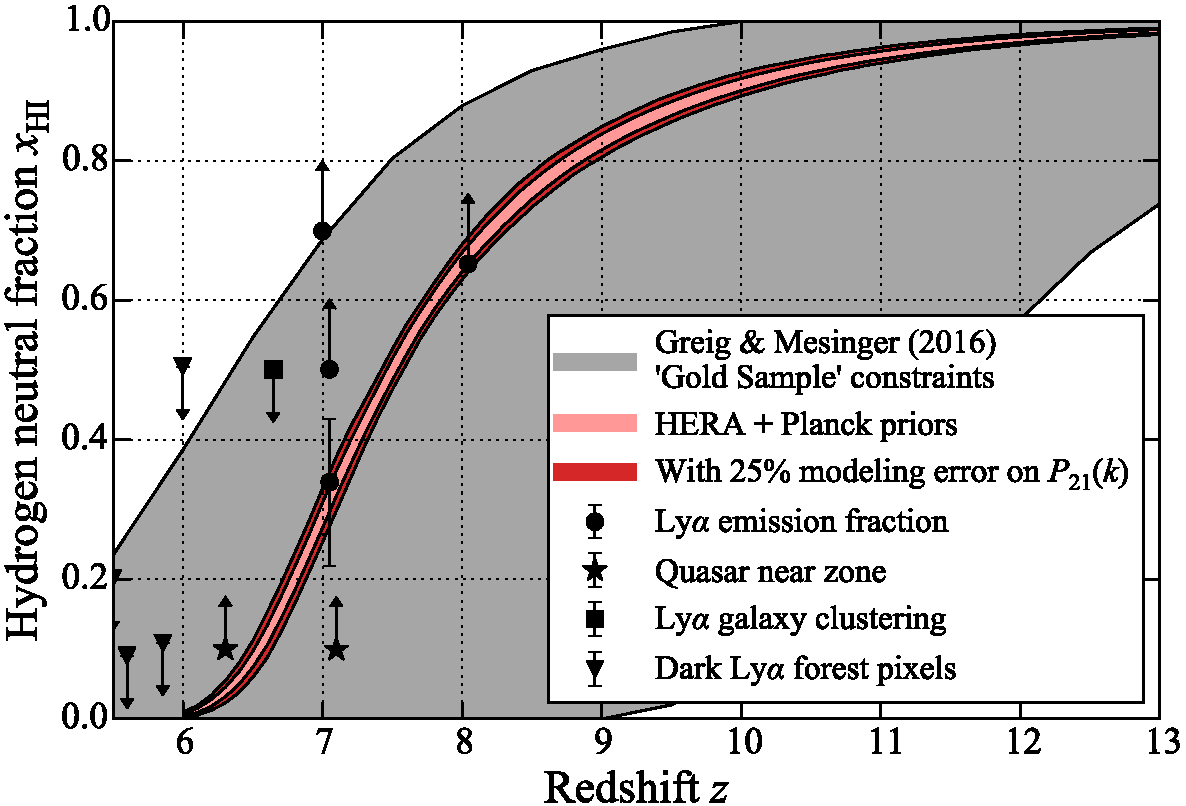
\includegraphics[width=0.51\textwidth,clip]{plots/ionHist.pdf}
  \caption{Combining direct constraints on $x_\text{HI}$, the hydrogen neutral fraction, as a function of redshift (black points) with \emph{Planck} priors yields
an inferred $95\%$ confidence region (gray).  HERA constraints with (dark red) and without (pale red) 
a conservative $25\%$ modeling error in the $21\,\textrm{cm}$ power spectrum can dramatically narrow this confidence region.}
	\label{fig:IonHist}
\end{figure} 



As shown in Figure~\ref{fig:IonHist},
existing probes are limited in
their ability to constrain reionization, and will be for the foreseeable future.
HERA will use
another complementary probe --- the 21\,cm ``spin-flip" transition of neutral hydrogen
--- to bring transformative new capabilities in this area.  The next sub-sections outline these goals.


\subsection{Precision Constraints on Reionization}
\label{sec:EoRPowerSpectra}


\noindent HERA's top science goal is to transform our understanding of the first stars, galaxies, 
and black holes, and their role in driving reionization. 
Through power-spectral measurements of the 21\,cm line of hydrogen in the primordial IGM,
HERA directly constrains the topology and evolution of reionization, 
opening a unique window into the complex astrophysical interplay between the 
first luminous objects and their environments.
Using cosmological redshift, HERA can associate 
the signal at each observing frequency with emission time (or distance) to determine both the time evolution
and three-dimensional spatial structure of ionization in the IGM.
This 3D structure encodes information about the clustering properties of galaxies,
allowing us to distinguish between models, even if they predict the same ionized fraction. 
With a new telescope optimized for 3D power-spectral measurements and with support for theoretical
modeling efforts, the HERA program will advance our understanding of early galaxy formation and cosmic reionization.


\begin{figure}[h!]
\centering
    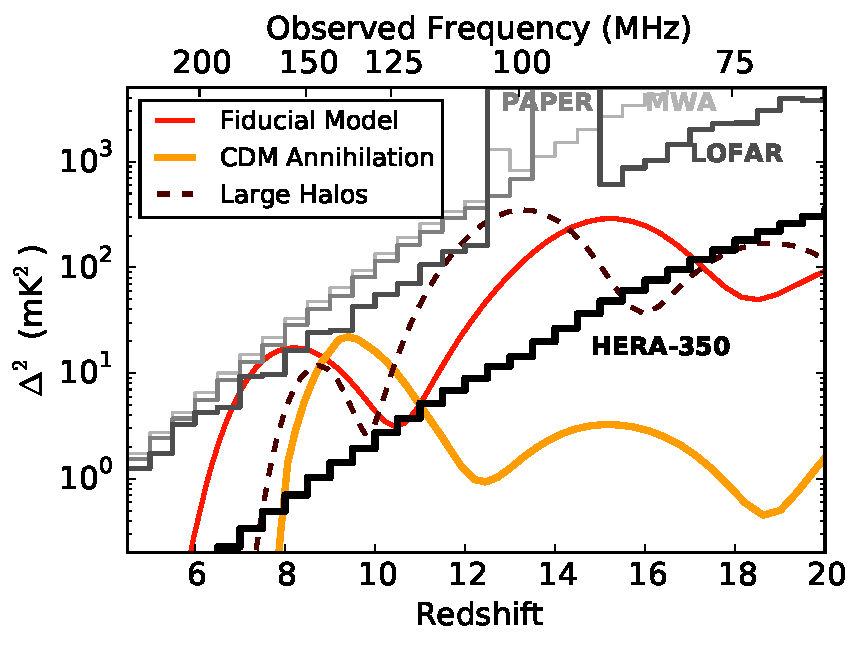
\includegraphics[width=0.49\textwidth,clip]{plots/sensitivity_wideband.pdf}
  \caption{ 1$\sigma$ thermal noise errors on $\Delta^2(k)$, the 21\,cm power spectrum, at $k\!=\!0.2$\,$h$\,Mpc$^{-1}$ (the dominant error at that $k$)
with 1080 hours of integration (black)
compared with various heating and reionization models (colored).}
	\label{fig:Sensitivities}
\end{figure}

HERA builds on the advances of first-generation
21\,cm EoR experiments led by HERA team members, particularly 
the Donald C. Backer Precision Array for Probing the Epoch of Reionization (PAPER; \citealt{parsons_et_al2010}),
the Murchison Widefield Array (MWA; \citealt{bowman_et_al2012,tingay_et_al2013}),
the MIT EoR experiment (MITEoR; \citealt{zheng_et_al2014}) and the Experiment to Detect the Global EoR Step (EDGES; \citealt{bowman_rogers2010}).  
Efforts by members of the HERA team
have produced the first astrophysically constraining upper limits on the 21\,cm EoR power spectrum, 
providing evidence for significant heating in the IGM prior to reionization \citep{parsons_etal2014,ali_et_al2015,pober_et_al2015}.
However, current experiments cannot expect more than marginal detections of the EoR signal. 
Figure~\ref{fig:Sensitivities} compares telescope sensitivities as a function of redshift to models of 
the evolving, spherically averaged 21\,cm EoR power spectrum $\Delta^2 (k) \equiv k^3 P(k) / 2 \pi^2$ (discussed later).  In contrast to current experiments,
HERA's optimized design and collecting area make it capable of
high-significance detections of virtually any realistic reionization scenario, even using only currently demonstrated foreground
mitigation strategies (see Table~\ref{tab:signif}). The development of enhanced foreground modeling and subtraction further improve the achievable constraints.


\begin{SCtable}
\caption{\hspace{-1.2mm}: Predicted SNRs of 21\,cm experiments for an EoR model with 50\% ionization at $z=9.5$, with 1080 hours observation, integrated over a $\Delta z$ of $0.8$.
Foreground avoidance represents an analysis comparable to \cite{ali_et_al2015}, whereas foreground modeling allows signifcantly more $k$ modes of the cosmological signal to be recovered.}
\small
 \centering
 \begin{tabular}{c||r||r|r} 
%\begin{deluxetable}{c||r||r|r}
%\tabletypesize{\small}
%\tablecaption{\small
\hline
%\startdata
Instrument & \shortstack{Collecting \\ Area (m$^2$)} & \shortstack{Foreground \\Avoidance} & \shortstack{Foreground \\Modeling} \\
\hline
PAPER & 1,188 & 0.77$\sigma$ & 3.04$\sigma$ \\
MWA & 3,584 & 0.31$\sigma$ & 1.63$\sigma$ \\
LOFAR NL Core & 35,762 & 0.38$\sigma$ & 5.36$\sigma$ \\
%\textbf{HERA-127} & \textbf{19,500} & \textbf{10.88} & \textbf{35.65} \\
\textbf{HERA-350} & \textbf{53,878} & \textbf{23.34$\sigma$} & \textbf{90.97}$\boldsymbol{\sigma}$ \\
SKA1 Low Core & 416,595 & 13.4$\sigma$ & 109.90$\sigma$
%\enddata
\end{tabular}
%\Caption{-0.1in}{0.99}{-0.1in}
\hspace{-0.1in}
\label{tab:signif}
\end{SCtable}

\begin{figure}[h!]
\centering
    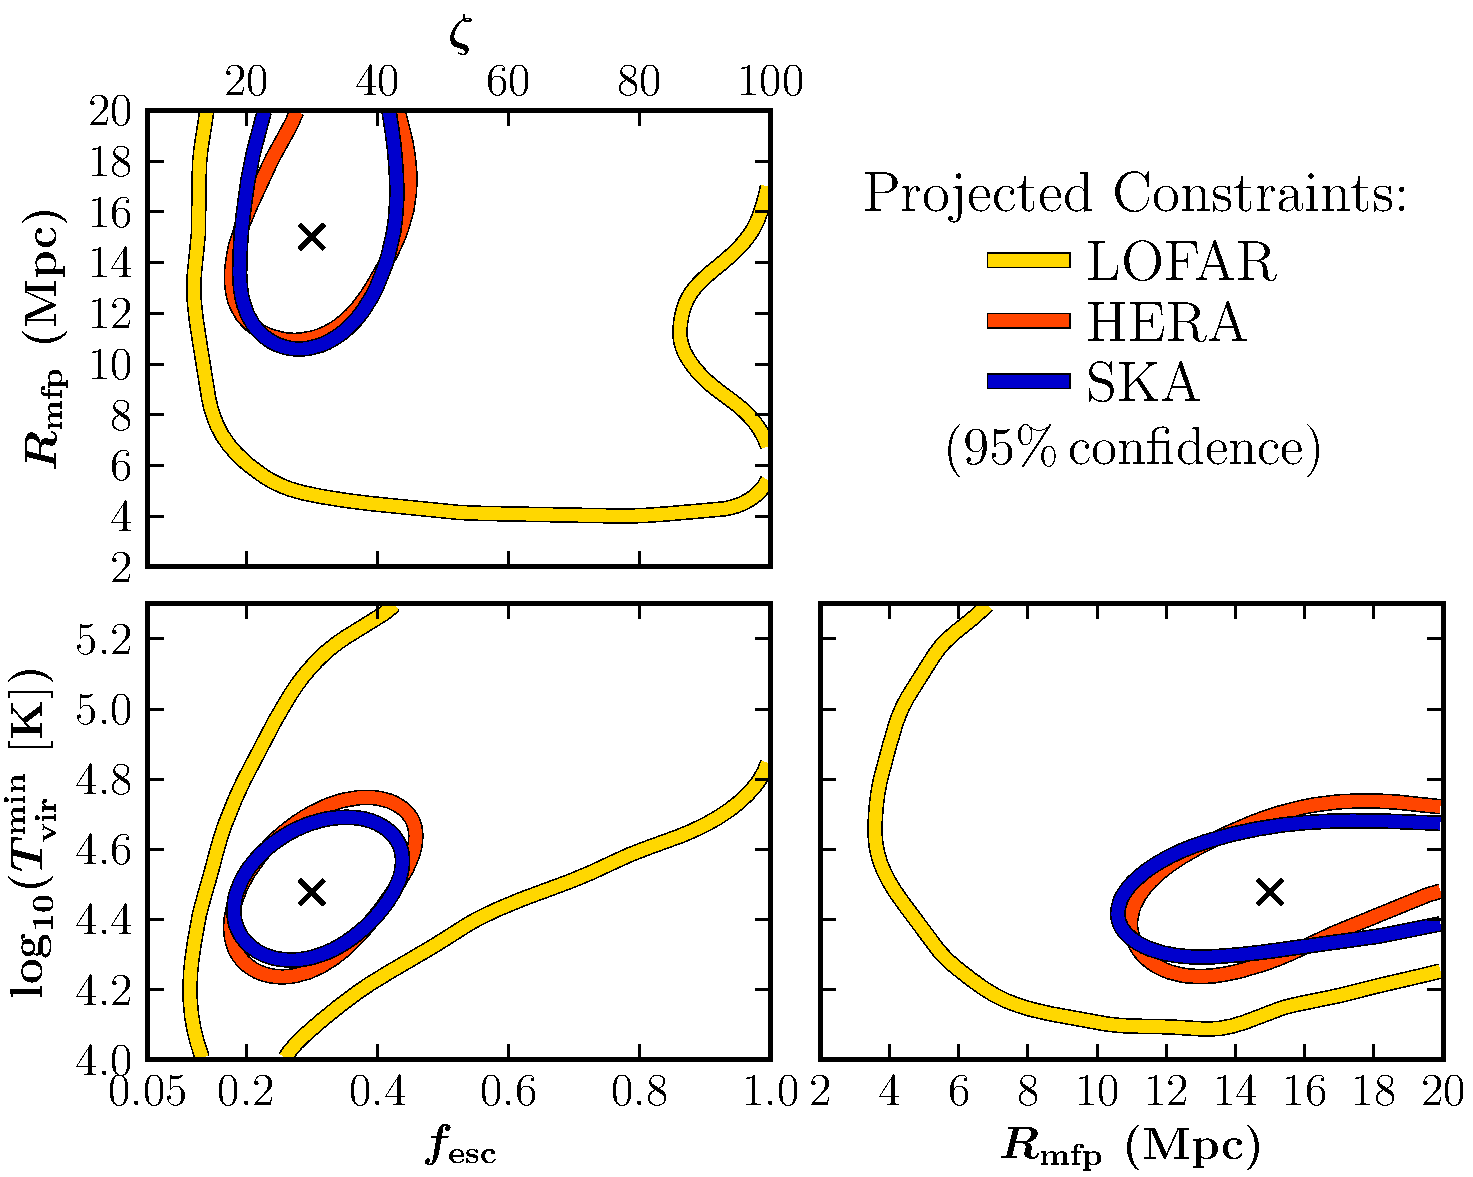
\includegraphics[width=0.56\textwidth,clip]{plots/LikelihoodContours_smaller_avoid_All3_no_table}
  \caption{Projected likelihood contours from an MCMC analysis for astrophysical parameters of reionization. Model parameters are $T_\textrm{vir}^\textrm{min}$ (minimum virial temperature of ionizing galaxies); $R_\textrm{mfp}$ (mean free path of ionizing photons in HII regions); and $\zeta_0$ (ionizing efficiency of galaxies).  Also shown are constraints on the derived ionizing escape fraction, $f_\textrm{esc}$. }
	\label{fig:paramConstraints}
\end{figure}
 
HERA's 21\,cm measurements can be used in conjunction with our semi-analytic models to constrain the ionization history. 
The red band in Fig.~\ref{fig:IonHist} shows the forecasted 95\% confidence region derived from HERA data after marginalizing over astrophysical and cosmological parameters.
Figure~\ref{fig:paramConstraints} shows the results of a Markov Chain Monte
Carlo (MCMC) pipeline for fitting models to 21\,cm power spectrum data \citep{greig_and_mesinger2015}, which we have conservatively limited to the range $8 < z < 10$ (although in practice a much broader bandwidth will be available; see Table \ref{tab:BasicParameters}).
Based on the excursion-set formalism of
\citet{furlanetto_et_al2004} and the 21cmFAST code \citep{mesinger_et_al2011},
this code models the astrophysics of
reionization with three free parameters (see Figure~\ref{fig:paramConstraints} for details). 
While the existing experiment with the most collecting area, 
the LOw Frequency ARray (LOFAR; \citealt{yatawatta_et_al2013}),
faces large
uncertainties, 
HERA's tight constraints on these parameters are comparable
to what could be achieved with the SKA.  Such results would be valuable for
informing the design and science case of the low-frequency SKA, highlighting areas where the SKA has unique capability.
Additionally, HERA's constraints enable principal component parameterizations of the
sky-averaged $21\,\textrm{cm}$ signal measurements pursued by experiments such as EDGES, increasing their signal-to-noise and thus their science return \citep{liu_parsons2015}.

\subsection{Existing Measurements}
\label{sec:existing}
PAPER adopted a foreground mitigation strategy based largely
on filtering out the wedge in frequency domain (so-called ``delay filtering"; \citealt{parsons_et_al2012b}).  
By reducing the need
for image-domain foreground modeling, this approach allowed PAPER to switch to a grid-based antenna layout that
enhanced sensitivity toward fewer Fourier modes and facilitated calibration
based on the ``redundancy" of different antenna pairs measuring the same sky modes \citep{zheng_et_al2014}.
Combined, redundancy and delay filtering provide a robust, inexpensive, and demonstrably successful solution 
to the foreground problem.  
Yet PAPER's lack of imaging support and its uneven $uv$ sampling 
leave it with limited diagnostic capability, particularly for direction-dependent systematics
such as polarization leakage from Faraday-rotated emission \Mycitep{moore_et_al2013}.
While concern over such effects has decreased markedly since discovering that
intrinsic point source polarization is lower than previously thought
\citep{asad_et_al2015} and that variable Faraday rotation through the
ionosphere averages down the polarized signal over long observing seasons
\Mycitep{moore_et_al2016}, direction-dependent beam effects remain an area of interest.
The MWA's image-based calibration and foreground subtraction strategy provides complementary
capabilities. Imaging with subtraction, while still under development as a viable foreground strategy,
can increase sensitivity by recovering more modes of the cosmological signal (see
Table~\ref{tab:signif}) and help address systematic errors rooted
in the image domain.  HERA's antenna configuration---shown in Figure \ref{fig:arrayConfig} and discussed in \S\ref{sec:arrayConfig}---emphasizes
the proven approaches of redundant calibration and delay filtering, while simultaneously
increasing the extent and density of $uv$ sampling for high-fidelity imaging.  

\begin{figure}[t]
	\centering
	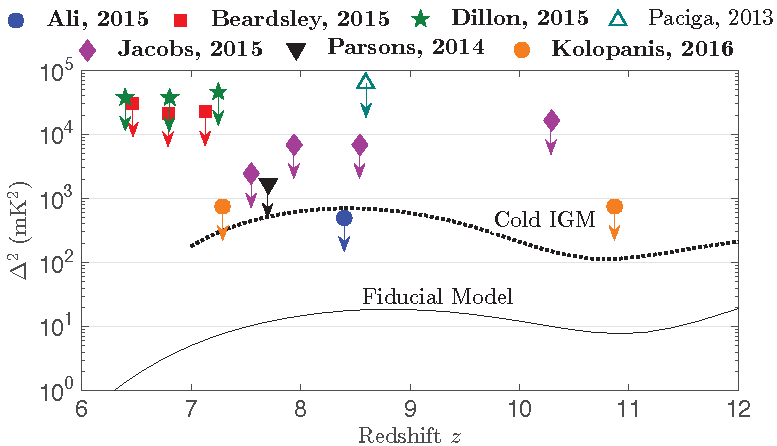
\includegraphics[width=.8\textwidth]{plots/current_limits.pdf}
	\caption{The current best published $2\sigma$ upper limits on the 21cm power spectrum, $\Delta^2(k)$, (solid symbols represent analyses led by HERA collaborators) compared to 21cmFAST-generated models at $k=0.2$\,$h$\,Mpc$^{-1}$. 
Analysis is still underway on PAPER and MWA observations that approach their projected 
full sensitivities (see Fig.~\ref{fig:Sensitivities}); 
HERA can deliver sub-$\text{mK}^2$ sensitivities.}
	\vspace{-10pt}
	\label{fig:limits}
	\label{fig:IGMtemperatureConstraints}
\end{figure}

Despite progress, the fact remains that the 21\,cm EoR signal is intrinsically very faint; making a detection requires a
large instrumental collecting area and a long, dedicated observing campaign.
Although published PAPER and MWA results (Fig. \ref{fig:limits}) do not yet include observations 
at full sensitivity that are still being analyzed (e.g. Fig. \ref{fig:Sensitivities}), 
it is clear already that these instruments lack the sensitivity
to make a conclusive detection (see Table~\ref{tab:signif}). 
HERA addresses this shortcoming with a dish element that delivers a much larger collecting area 
while retaining the necessary characteristics for both proven and forward-looking foreground removal strategies.

\subsection{Secondary Scientific Objectives}%\\Precision Cosmology, Reionization Imaging, and High-$z$ IGM X-Ray Heating Science}

\startsquarepar\emph{\textbf{Precision Cosmology.}}
\label{sec:tau}
By advancing our understanding of reionization astrophysics, HERA improves CMB constraints on 
fundamental cosmological parameters by
removing the optical depth
$\tau$ as a nuisance parameter. HERA breaks the degeneracy between the
constraints on $\tau$ and the sum of the neutrino masses $\sum m_\nu$, which has
been identified as a potential problem for Stage 4 CMB lensing experiments. A
HERA-informed estimate of $\tau$ enables CMB lensing experiments to achieve a
$0.012\,\textrm{eV}$ error on $\sum m_\nu$ \citep{liu_et_al2015}. This would
represent a $\sim$5$\sigma$ cosmological detection of the neutrino masses even
under the most pessimistic assumptions
% that their sum is the minimum value of $0.058\,\textrm{eV}$ 
still allowed by neutrino oscillation \stopsquarepar

\begin{figure}[h!]
\centering
    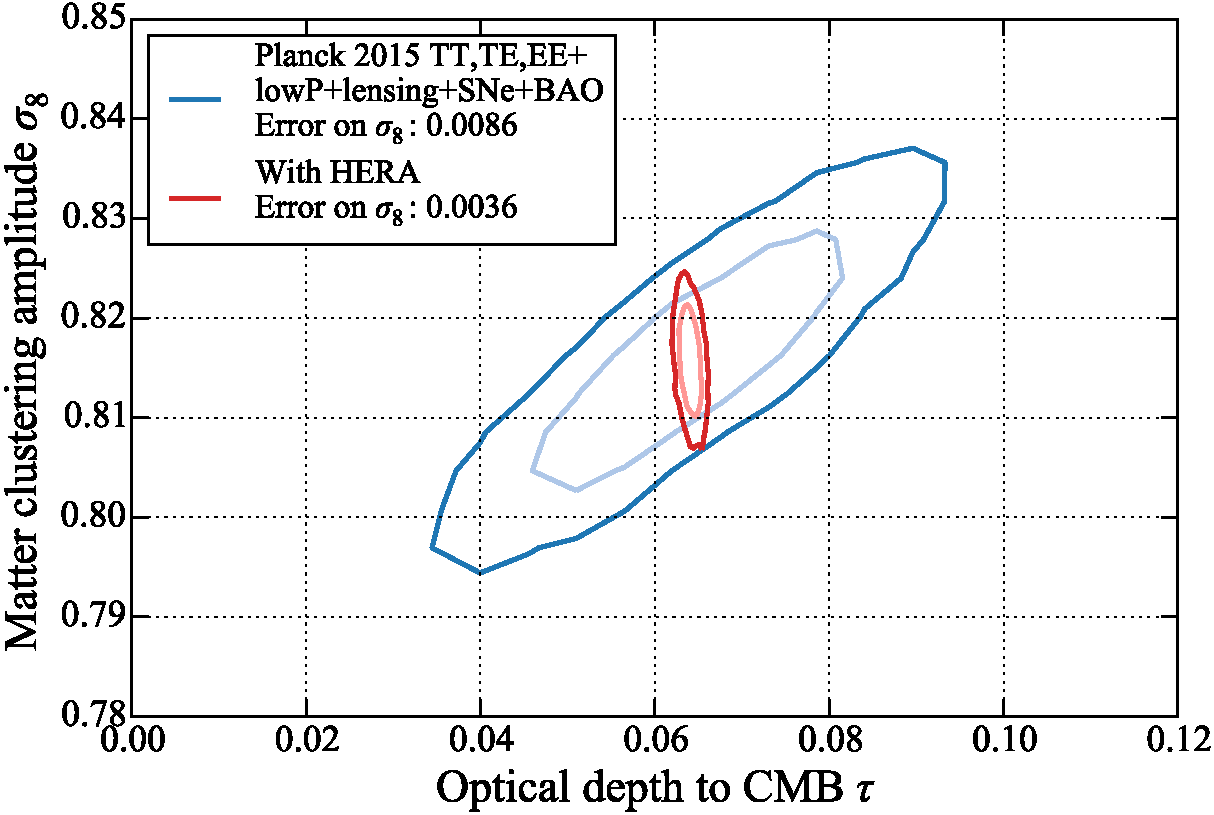
\includegraphics[width=0.50\textwidth,clip]{plots/sigmaTau.pdf}
\caption{Likelihood contours ($68\%$ and $95\%$) for $\sigma_8$ and $\tau$ using \emph{Planck} constraints (blue) and 
adding HERA data (red). 
%Light and heavy contours signify $68\%$ and $95\%$ confidence regions, respectively. 
The $21\,\textrm{cm}$ constraints break the CMB degeneracy between the amplitude of density fluctuations and the optical depth, improving constraints on both.}
	\label{fig:sigma8Tau}
\end{figure} 

\noindent experiments
\citep{allison_et_al2015}, making HERA key to our understanding of neutrino
physics. HERA's estimate of $\tau$ would also break the degeneracy between
$\tau$ and the amplitude of matter fluctuations (expressed in Fig.
\ref{fig:sigma8Tau} as $\sigma_8$) that arises when using only
CMB data. HERA effectively reduces error bars on $\sigma_8$ by more
than a factor of three \citep{liu_et_al2015}, potentially elucidating
current tensions between cluster cosmology constraints and those from primary
CMB anisotropies.

\emph{\textbf{First Images of the Reionization Epoch.}}
\label{sec:imaging}
In addition to measuring the power spectrum, HERA has sufficient 
sensitivity to directly image the IGM during reionization,
and will observe a 1440 deg$^2$ stripe, comparable to future WFIRST
large area near-IR surveys.
 After 100 hours on a
single field (achievable in 200 nights), HERA reaches a surface brightness 
sensitivity of 50 $\mu$Jy/beam (synthesized beam FWHM $\sim$ 24$'$) compared 
to the brightness temperature fluctuations of up to 400 $\mu$Jy/beam in typical 
reionization models (see Fig.~\ref{fig:LSS}). From the standpoint of sensitivity alone, HERA is capable of 
detecting the brightest structures at $z=8$ with SNR $>$ 10. Additionally, the design 
of HERA places it in a unique position to directly explore calibration techniques
(e.g. redundant calibration, \citealt{liu_et_al2010}), while retaining a high quality 
point spread functions for imaging and identifying foregrounds. Leveraging the expertise gained 
through both precursor strategies, HERA will yield exceptionally high dynamic range
images.

%\subsubsection{The 21\,cm Signal in the Pre-Reionization Epoch}

%\begin{wrapfigure}{R}{0.5\textwidth}
\begin{figure}[b!]
\centering
\vspace{-15pt}
    %\includegraphics[width=.5\textwidth,clip]{plots/imaging/HERA_z8_SNR_annotated_2015.png}
    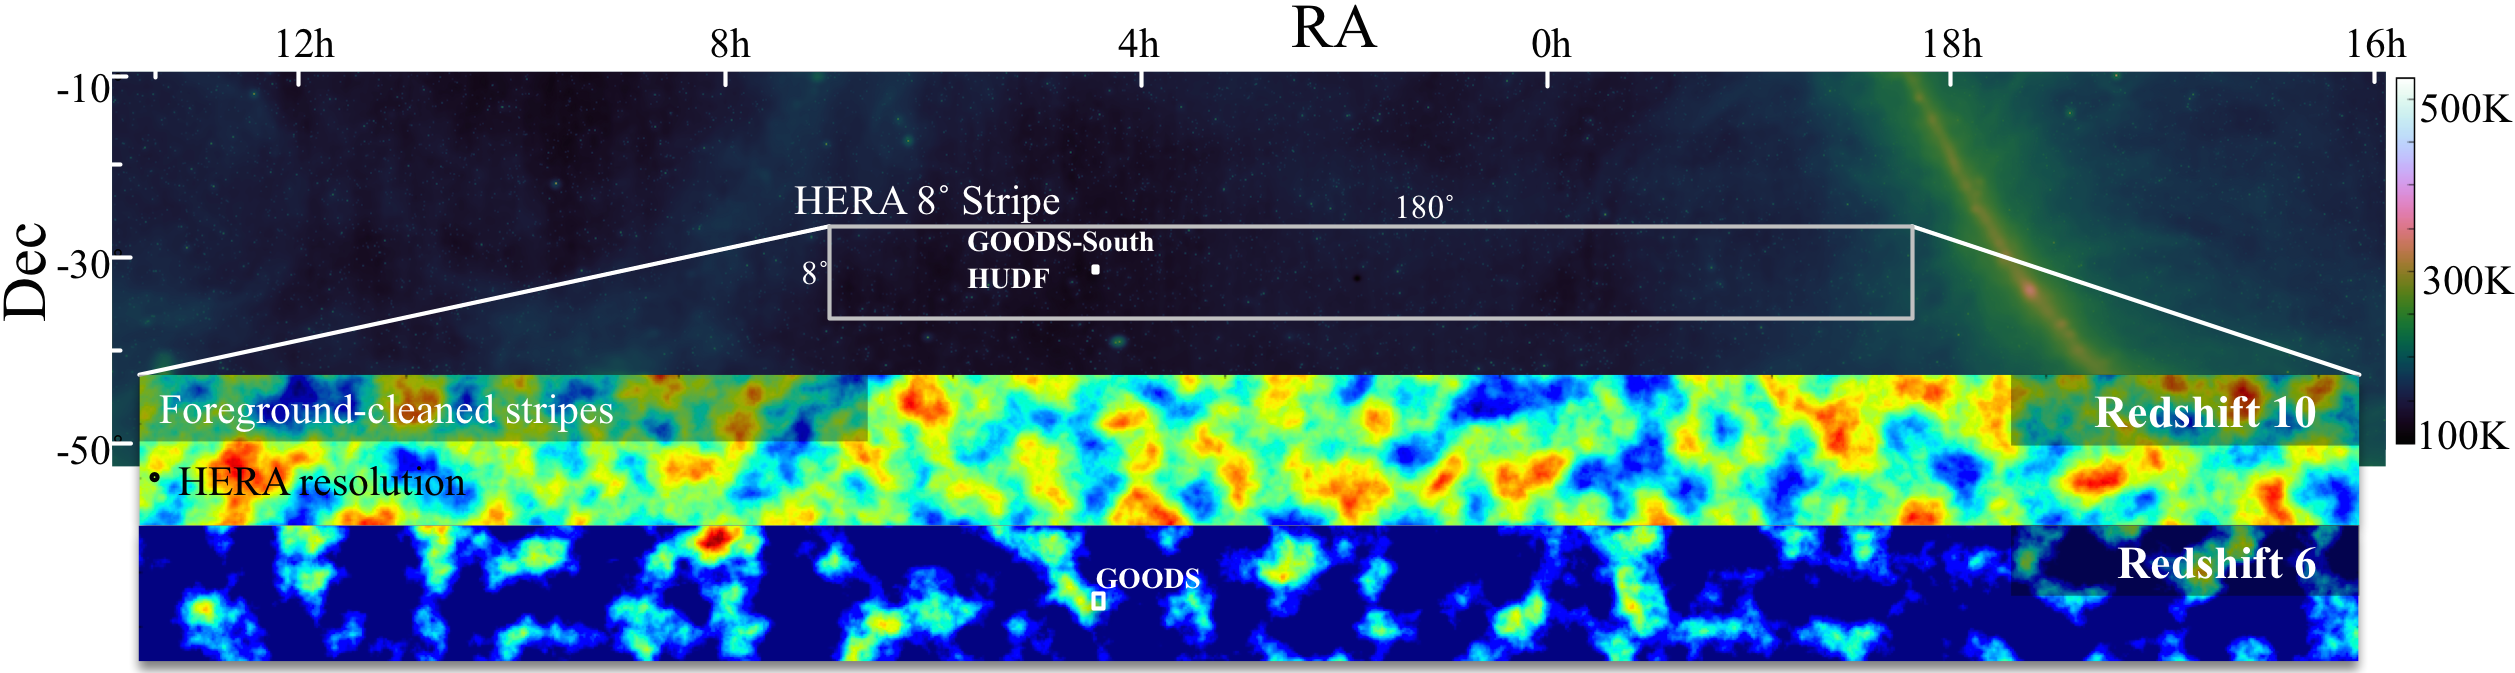
\includegraphics[width=1.0\textwidth,clip]{plots/HERA_FoV_w_strips.png}
  \vspace{-20pt}
\caption{\footnotesize 
HERA will observe a 1440 deg$^2$ stripe centered near $\delta = -30^\circ$. HERA can measure the ionization state around galaxies in, e.g., the GOODS-South field that contains a third of all known $z\!>\!8$ galaxies. HERA's primary imaging data product to the community will be deep cubes along the HERA stripe suitable for cross-correlation.
\label{fig:LSS} }
\vspace{-10pt}
\end{figure}
%  \vspace{-10pt}
%\end{wrapfigure}

\emph{\textbf{Pre-Reionization Heating.}}
\label{sec:EoX} 
Prior to reionization, the 21\,cm signal is a sensitive probe of the first
luminous sources and IGM heating mechanisms. First stars are expected to form
at $z \sim 25-30$ and their imprint on the 21\,cm signal is expected to be
sensitive to the halo mass where they are formed \citep{mesinger_et_al2015}.
The IGM is then expected to be heated by first
generation X--ray binaries
\citep{furlanetto_et_al2006_global,pritchard_et_al2007,mesinger_et_al2013} or
by the hot interstellar medium produced by the first supernovae
\citep{pacucci_et_al2014}, although the heating timing and magnitude is still
very much debated \citep{fialkov_et_al2012}. Dark matter annihilation
\citep{evoli_et_al2014} could also inject energy in the IGM, leaving its
imprint in the 21\,cm signal.
 
With support from the Moore Foundation to develop feeds sensitive down to 50\,MHz, HERA will probe the IGM prior to
reionization and constrain the sources of heating, obtaining, in the case of
X--ray heating, percent-level constraints on the efficiency with which star-forming baryons
produce X-rays \citep{ewall-wice_et_al2015}. While the observational and analytical state of the art of pre-reionization 21\,cm science is not as advanced as for the EoR \citep{ewall-wice_et_al2016-EoXLimits}, the risk of lower-frequency observing is borne by the Moore Foundation.
Lower
frequency observations also test feedback
mechanisms that interact with low-mass halos at high redshifts
\citep{Iliev_et_al2007,Iliev_et_al2012,ahn_et_al2012}.
Such constraints, while interesting in their own right, also reduce
the susceptibility of the aforementioned $21\,\textrm{cm}$-derived $\tau$
constraints to uncertainties in high-redshift physics \citep{liu_et_al2015}, especially if they are 
combined with upcoming or proposed measurements of 
the pre-reionization sky-averaged spectrum \citep{fialkov_and_loeb2016}. Additionally, they may be crucial to a correct
interpretation of kinetic Sunyaev-Zel'dovich effect constraints on reionization
from the CMB \citep{park_et_al2013}. The high redshift probe of
structure afforded by the low frequency $21\,\textrm{cm}$ measurements will
permit some of the most direct observations of hypothesized suppressions of
small-scale structure
\citep{dalal_et_al2010,tseliakhovich_et_al2011,fialkov_et_al2012} arising from
predicted supersonic relative velocities between dark matter and baryonic gas
\citep{tseliakhovich_and_hirata2010}. No other electromagnetic probe can provide direct observations of this
epoch. 


\subsection{Other Scientific Objectives}
\label{subsec:broader_science}

\noindent With unprecedented sensitivity at this frequency range, HERA can deliver much more than its core 21\,cm science. 
Some of HERA's broader science impacts derive directly from the public data products HERA delivers.  Other
areas of impact may require additional hardware or software that HERA can host at no extra risk. 
In this respect, HERA serves as a ``platform" for additional science programs with external funding.
The Moore Foundation's support of HERA feed development and data analysis targeting the pre-reionization science described in \S\ref{sec:EoX}
is a prime example of how we envision this functioning.
Below, we list examples of the broader science that HERA can deliver.

\emph{\textbf{Cross-Correlations with Other Reionization Probes.}}
\label{sec:crossCorr}
HERA's public data provide new opportunities for cross-correlation studies.
Cross-correlation between HERA 21\,cm images and other high-redshift probes
(e.g. JWST; WFIRST; CMB maps; CO, CII, and Ly-$\alpha$ intensity mapping) 
can provide an independent confirmation of the 21\,cm power spectrum
\citep[i.e.][]{lidz_et_al2009,dore_et_al2014,silva_et_al2015,vrbanec2016} and enable rich new studies of
the interaction between galaxies and their ionization environment. 
In particular, cross-correlating 21\,cm with galaxy surveys can measure the characteristic bubble size around galaxies of
different luminosities \citep{lidz_et_al2009} and help separate the degeneracy
between the fraction of photons escaping the galaxies and the
total number of ionizing photons produced \citep{zackrisson2013}.

HERA is placed in a unique position to enable such cross-correlation: the GOODS-South field---one of the most panchromatically studied regions of the sky, the site of the Hubble UDF, and home to over a third of all known $z>9$
galaxies---lies in its field of view. HERA's images of the IGM can provide environmental context to galaxy surveys through identification of
ionized bubbles \citep{malloy_lidz2013}, or in a more statistical sense as
described in \cite{beardsley_et_al2015}. 


\textbf{\emph{Searching for Exoplanetary Radio Bursts.}}
\label{sec:exoplanets}
HERA could be an powerful tool in the search for bright, highly polarized auroral bursts
from exoplanets %due to the electron cyclotron maser instability 
\citep{treumann2006,hallinan_et_al2015}. These
distinctive, coherent bursts occur periodically at the planetary
rotation rate, which cannot otherwise be measured. 
A burst from a terrestrial planet could point toward
habitability, since it implies a powerful magnetic field
protecting the atmosphere and perhaps the biosphere from energetic stellar wind
particles \citep{tarter_et_al2007}. HERA's sensitivity, large FoV, long campaigns, and precise calibration are all well-suited
for discovering exoplanetary radio bursts from Jupiter-like planets out to 25~pc. Many well studied exoplanetary systems within that distance are in the HERA stripe, including Fomalhaut, Gl 667 C, Gl 433, HD 147513, and Gl 317.


\textbf{\emph{Fast Radio Burst Followup.}}
\label{sec:FRBs}
Fast Radio Bursts (FRB) are millisecond-long radio flashes whose origin has remained a great enigma ever since their discovery \citep{2007Sci...318..777L}. 
If equipped with a suitable backend, HERA could be triggered by nearby, higher-frequency telescopes for FRB followup, saving baseband data and thus full sensitivity to all dispersion measures.
Bursts like that discovered by \citet{masui_et_al2015}, the lowest frequency
FRB detection to date, should be seen hourly by HERA at 5--10$\sigma$. %(including the effects of scattering)
 Observations at HERA frequencies are very sensitive to the physics of
the intervening medium, particularly deviations from $\lambda^2$
dispersion. Detecting deviations would rule out broad classes of models and could indicate whether FRBs are at cosmological distances.

\section{Measuring the EOR}
\label{sec:eormeas}
Due to the expansion of the Universe over cosmological time, we can identify and measure the early Universe via the red-shift of spectral lines.  The hydrogen hyperfine transition at a rest frequency of 1420 MHz is a key spectral line due to the ubiquity of hydrogen and, being a ``forbidden'' transition, the optical depth lets us see through the entire Universe back almost to the period of recombination.  The bandwidth
therefore equates to a cosmic volume along the site of the telescope, with the frequency determining the cosmic age.

Given the difficulty of the experiment, initial measurements of the EOR strive to measure a statistical power spectrum of the signal since the nature of the reionization process should have a specific spatial signature.  The goal is therefore to measure a range of aggregate spatial scales on the sky, rather than to image the signal directly.  Imaging does remain an ultimate goal to fully understand the process, however we will need a greater understanding of the full measurements to achieve this more difficult goal.  MANY PAPERS, see Nithya and Jonnie recent

Obviously between our present observation point and the Epoch of Reionization approximately 13 billion years ago lies the entire intervening Universe, which has an intrinsically much brighter signal (up to 6 orders of magnitude or more).  Primarily, this power is due to diffuse Galactic synchrotron radiation, supernova remnants and extragalactic radio sources.  As a first step, areas of the sky with where these signals are minimal (for example, outside the galactic plane and away from strong point sources) are targeted (REF FOR THIS).  More importantly and most fortuitously however is the fact that all of these foreground signals are smooth spectrum sources whereas the expected spectrum of the EOR is expected to be rough since it is made up of non-ionized regions which are randomly distributed over a wide range of redshifts.  This fact allows us to try and isolate foregrounds from the EOR, as will be discussed.

This section will provide a brief overview of existing measurements and the theoretical underpinning of how foregrounds contaminate the measurement (the so-called ``wedge''), discuss the various techniques used to make the measurement and finally provide a brief discussion on calibration issues and techniques.

\subsection{The ``Wedge''}
The past three years have seen deep EoR observations with PAPER, the MWA, 
the Giant Metrewave Radio Telescope (GMRT; \citealt{paciga_et_al2013}), and LOFAR.
PAPER and the MWA have produced progressively deeper limits
\citep{dillon_et_al2015,parsons_etal2014,ali_et_al2015}, with PAPER
yielding the first meaningful constraints on the 21\,cm spin temperature during reionization
(Fig. \ref{fig:limits}).
The inherent challenge is to simultaneously meet stringent sensitivity requirements 
while suppressing foregrounds $\sim5$ orders of magnitude
brighter than the 21\,cm signal, which has been addressed along a number of approaches.  
To address this challenge,  all aspects of the experimental process must be refined and improved, spanning 
calibration ({\em e.g.} \cite{zheng_et_al2014, jacobs_et_al2016, barry_et_al2016}), handling foreground contamination
({\em e.g.} \cite{moore_et_al2013,moore_et_al2016,thyagarajan_et_al2015a,pober_et_al2016}),
and the interferometer design itself ({\em e.g.} \cite{parsons_et_al2012a,dillon_parsons2016}).

Perhaps the most important advance informing HERA's design is a
refined understanding of how smooth-spectrum foregrounds interact
with instrument chromaticity to produce a characteristic ``wedge" of
foreground leakage in Fourier space (see Fig.~\ref{fig:wedge}), 
outside of which the 21\,cm signal dominates.
Through theoretical and observational work
\citep{datta_etal2010,morales_et_al2012,parsons_et_al2012b,vedantham_2012,thyagarajan_et_al2013,hazelton_et_al2013,pober_etal2013b,liu_et_al2014a,liu_et_al2014b},
we have learned how the boundary between the wedge and our ``EoR window" is determined by the separation between antennas,
signal reflections within antennas, and the angular response of the antenna beam.  Deep integrations also show us
that, to the limits of current sensitivity, foreground emission is absent outside of the wedge; it can only 
appear there through instrumental leakage \citep{parsons_etal2014,ali_et_al2015,moore_et_al2016,kohn_et_al2016}.

Though the power spectrum measurement is over a volume, it is instructive to split the spatial wavenumbers into two components,  $\kvec =  \kvpr + \kpar{\hat {\bf z}}$ where $\kvpr$ is determined by the antenna baseline and $\kpar$ by the frequency.  This is useful since it allows us to split out the chromatic response of the interferometer and isolate a phase space where foreground sources ({\em i.e.} everything {\em not} the EOR) contaminate the signal of interest from where they don't.  This contaminated phase space may be shown [REF] to be a wedge-shaped region in $\kpr$:$\kpar$ space:
\begin{equation}
|\kpar| \le \beta\frac{X\lambda}{Yc}\kpr + \frac{S}{Y}
\end{equation}
where $c$ is the speed of light and $S$ is a parameter accounting for offsets related to the combined spectral smoothness of the foregrounds and the antenna response (see Fig. \ref{fig:wedge}).  
A key issue to measuring the EOR power spectrum is to understand and minimize such effects.  For an analytical derivation, see \cite{zahn_etal2012,vedantham_2012,liu_et_al2014b},  in simulation see \cite{datta_etal2010,hazelton_et_al2013} and for observations
\cite{pober_etal2013b,2015arXiv150601026P,parsons_etal2014,2015arXiv150206016A}.  Note that the unit of the spatial wavenumber $k$ is 1/length, in this case the relevant length scale is megaparsecs (Mpc; 1 Mpc = 3.086$\times10^{22}$ m).  In order to normalize for updated measurements of the Hubble constant, it is further normalized by a factor $h$, where Hubble's constant is expressed as $H_o=100h$ (km/s)/Mpc , such that the wavenumbers are expressed as $h$/Mpc.

\begin{figure}[t]
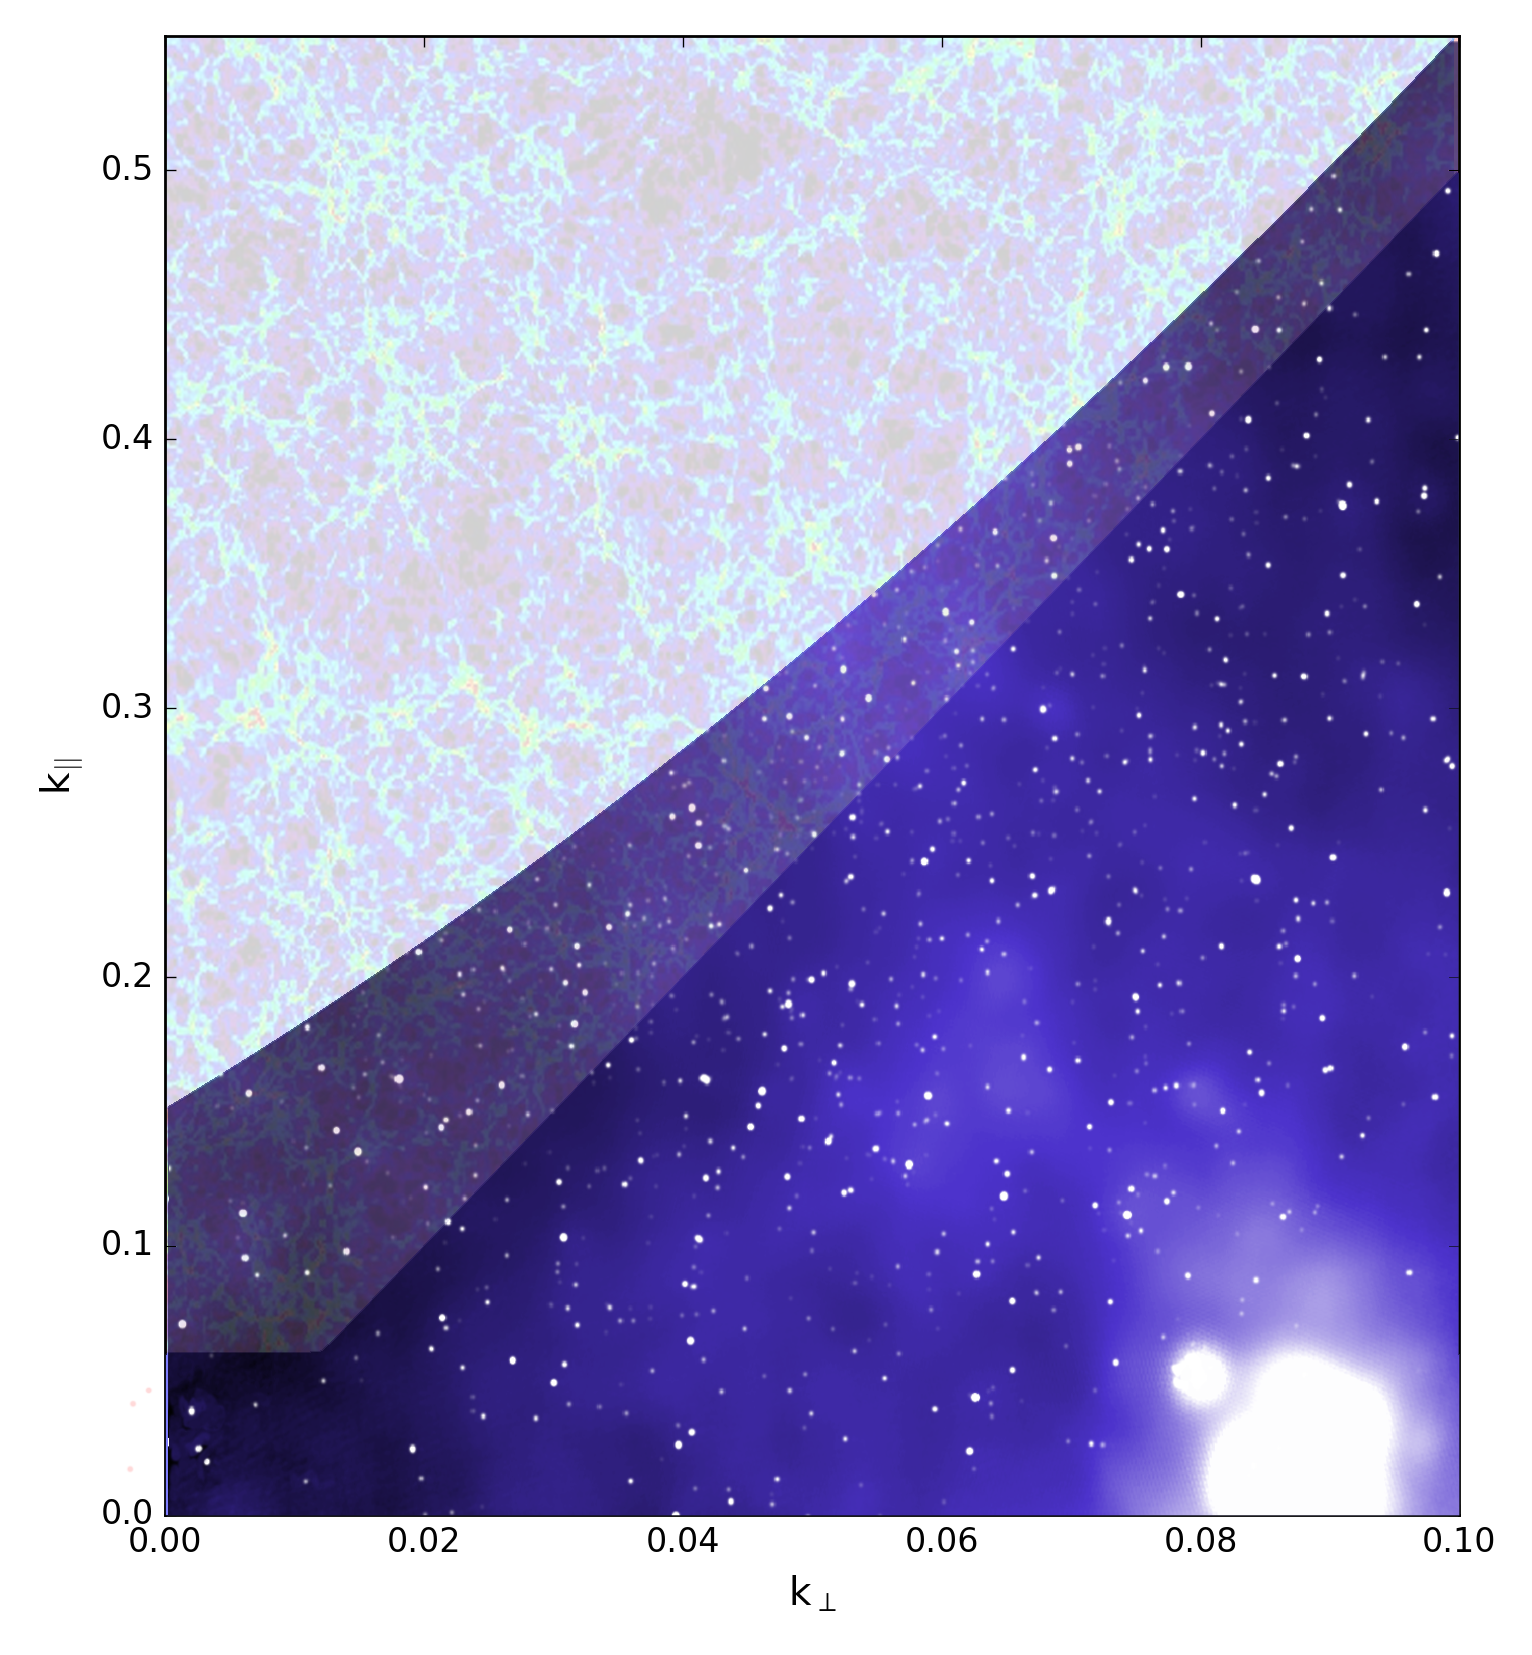
\includegraphics[height=3in]{plots/wedgeWithBG.png}
\caption{Foregrounds are a primary challenge facing 21\,cm cosmology experiments. 
HERA leverages a ``wedge'' in the spherically-averaged ($\mathbf{k}$ is broken into $k_\|$ and $k_\perp$) power spectrum (center panel; \citealt{dillon_et_al2015}). Smooth-spectrum foregrounds (right panel) $\sim$5 orders of magnitude brighter than fiducial EoR models (left panel; \citealt{mesinger_et_al2011}) create the ``wedge'' when they interact with the interferometer's chromatic response. By avoiding foregrounds, PAPER has placed limits within an order
of magnitude (in mK) of these models \citep{ali_et_al2015} and show the ``EoR Window'' to be foreground-free.
HERA's dish and configuration optimize wedge/window isolation and direct sensitivity to low-$k_\perp$ modes where EoR is brightest.
%v2
Cartoon of the wedge.  The gray rectangle represents the smooth-spectrum foregrounds as they would be if the instrument had a perfect achromatic response.  The pink wedge area shows the chromatic response of the interferometer, where additional power is thrown up from the gray region to higher k-values with increasing baseline.  The additional horizontal pink line illustrates the affect that other systematics, such as reflections on cables, can have in contaminating the measurement.  The white region shown the 'eor window', where the measurement is not contaminated by foregrounds or systematics.}
\label{fig:wedge}
\end{figure}

The techniques to measure the power spectrum may be broken down into two principle techniques (delay-space and map-making), plus additional hydrid methods.  These are briefly summarized below, with an emphasis on the delay-spectrum technique as the initial approach taken by HERA.  Finally, we provide a short discussion on calibration in the concept of this design.

\subsection{Delay-Spectrum Approach}
\label{sec:delayapproach}
Given that the response of an interferometer natively measures the power in Fourier modes of the sky within its beam, we see that it is a natural instrument to use for this measurement.  There are now numerous papers in the literature on the technique of measuring the power spectrum using an interferometer and the attendant issues [[[list of citations]]].  Below, a high-level overview based on  \cite{parsons_et_al2012b} will be presented. The so-called delay-spectrum approach leverages the interferometer measurement to optimize sensitivity to the desired modes while rejecting modes contaminated by the foreground power in the wedge.  Other than potentially handling overlapping bins in {\em uv} space, the delay-spectrum approach does not combine baselines before squaring and calculating the power spectrum.

We can essentially relate the sky power spectrum mode ${\hat P}(\kvec)$ to an interferometer baseline visibility ${\tilde V}(\bvec)$, which is the equivalent of the (complex) fringe pattern in a double slit experiment:
\begin{equation}
{\hat P}(\kvec) \approx\frac{X^2Y}{4k_B^2}   \left[\frac{{\tilde V}^2(\bvec)}{\Omega_b B/ \lambda^4} \right]
\label{eq:Pk_baseline}
\end{equation}
where $X$ and $Y$ are cosmological parameters relating angular size and spectral frequency to cosmic volumes (so, relating wavenumber to physical volume at a given redshift), $\Omega_b$ is the integrated beam response, $B$ is the effective bandwidth, $\lambda$ is the observation wavelength, and $k_B$ is Boltzmann's constant.  The terms in square brackets are instrumental terms, as opposed to the constants and cosmological parameters.  
Note that at the red-shifts of interest $X$ has a value of about 160 Mpc/deg and $Y$ has a value of about 16 Mpc/MHz.
Rather than ${\hat P}(\kvec)$, the literature generally works with a volume-normalized parameter given by $\Delta^2(k) = \frac{k^3}{2\pi^2}{\hat P}(\kvec)$.    

Since the thermal noise per visibility baseline may be expressed as
\begin{equation}
V_N = \left(\frac{2k_B}{\lambda^2}\right)\left(\frac{T_{sys}}{\sqrt{2B\tau}}\right)\Omega_b B
\label{eq:sensitivity_per_baseline}
\end{equation}
where $\tau$ is the integration time (see {\em e.g.} TMS),
to determine the sensitivity of an instrument to the power spectrum per baseline we can substitute the thermal noise per baseline for the visibility in Eq. \ref{eq:Pk_baseline}.  Further, since an interferometer typically measures many baselines which may be averaged together to improve the signal-to-noise per $k$-bin, the total sensitivity may be approximated as
\begin{equation}
\Delta^2_N (k,z)\approx \frac{k^3X^2(z)Y(z)}{4\pi^2} \left[\frac{T_{sys}^2(z)\Omega_b(z) }{\tau(z) \mathcal{N}_s(k)}\right]
\label{eq:sensitivity}
\end{equation}
where $\mathcal{N}$ represents the improvement in sensitivity based on the array configuration, which may significantly boost the sensitivity if optimized for this measurement 
(see \cite{parsons_et_al2012b}).  Fig. \ref{fig:boost} plots this ``boost'' factor for various telescopes under nominal observing campaigns using the delay-spectrum technique.  The large improvement for PAPER and HERA is the fact that the baselines are redundantly placed on appropriate spatial scales, so that a more limited number of unique baselines get sampled many times.



\begin{figure}[h!]
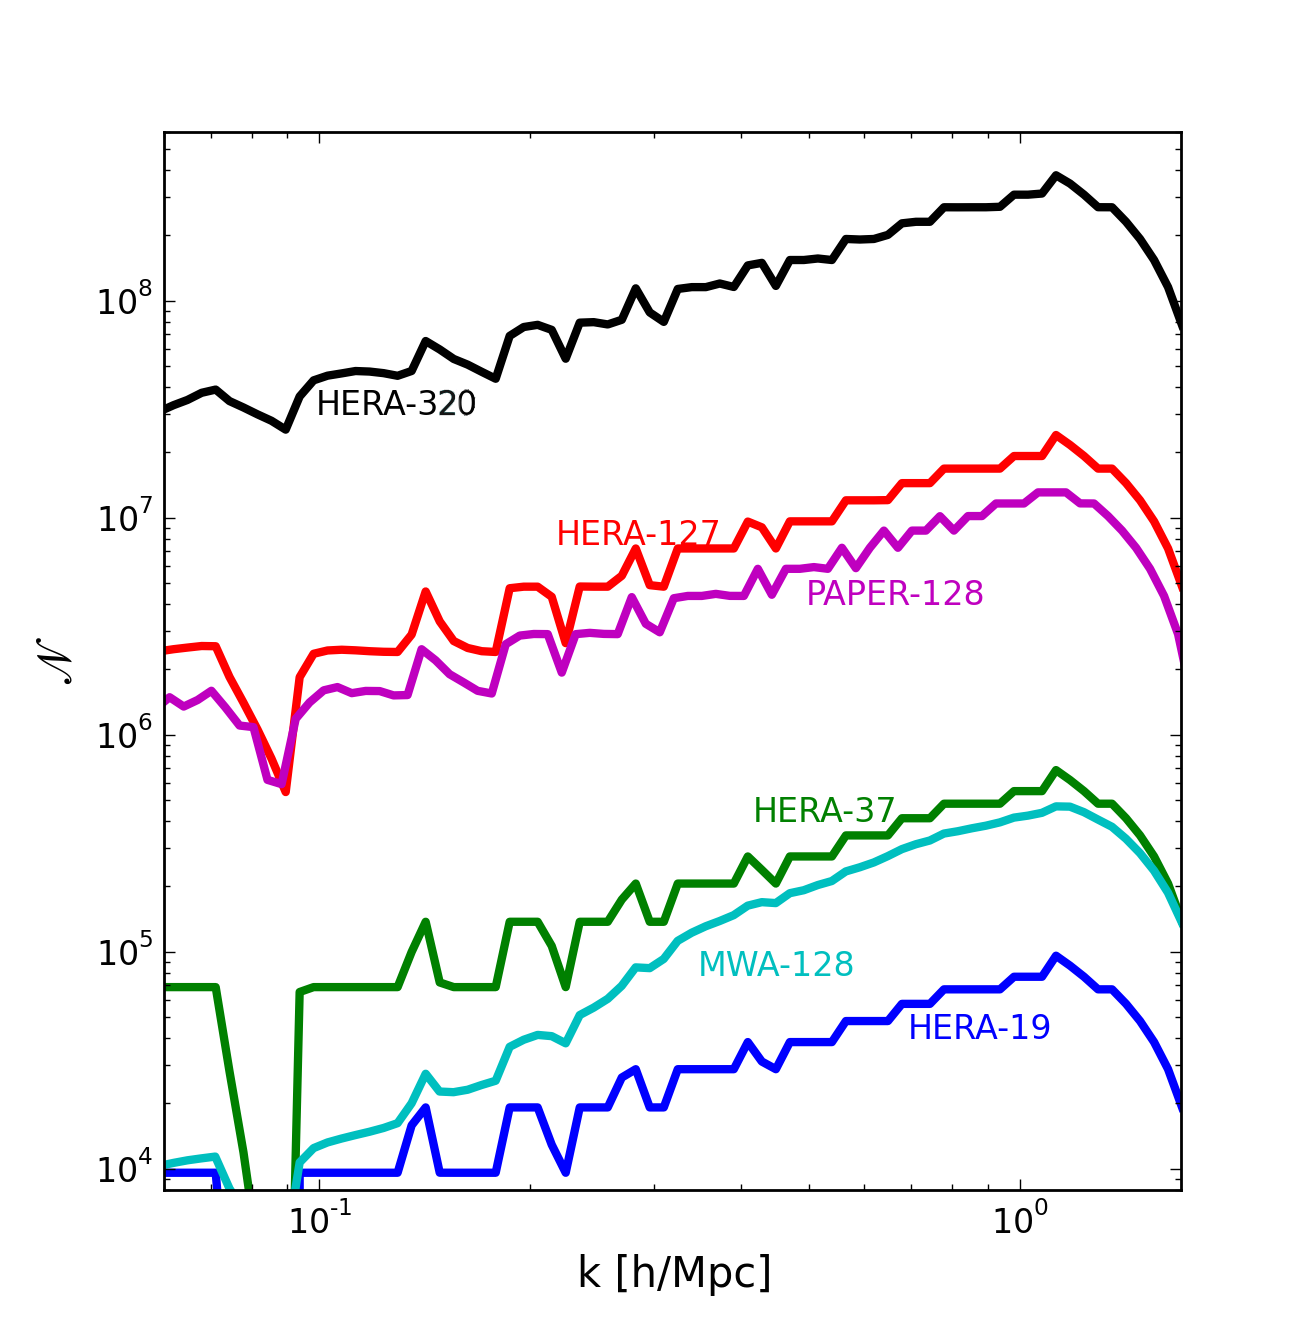
\includegraphics[width=0.5\textwidth]{plots/boost.png}
\caption{Representative boost factors ($\mathcal{N}$ in Eq. \ref{eq:sensitivity}) for representative observing campaigns for various instruments.
ADD NEW HERA CONFIGURATION AND LOFAR AND PUT IN 'HOW TO MAKE THIS PLOT'}
\label{fig:boost}
\end{figure}

The power spectrum uses the full magnitude of the {\bf k}-vector, which is set by the antenna baselines and bandwidths, as discussed above.  Note that cosmic evolution limits the largest bandwidth (which determines the smallest $\kpar$) to about 10 MHz -- for larger bandwidths the evolution of the Universe begins to impact the result.  For HERA, wavenumbers are dominated by the bandwidth, not the baseline.

Figure \ref{fig:kperf} is a rather busy plot showing many of the dependencies on wavenumber of bandwidth, configuration and the cosmos.  It shows the perpendicular, parallel and total resolution wavenumber as a function of redshift for various bandwidths and baselines.  The term {\em resolution} wavenumber is used, since it is a lower limit for that parameter since larger wavenumbers may be obtained at smaller bandwidths.  Blue lines denote $\kpar$ values, black lines denote $\kvpr$, and green lines denote total magnitude ($|{\bf k}|$) and the lines are labelled for the assumed bandwidth and/or baseline, depending on the type of wavenumber.  Obviously nearly any values may be used, but here a small sampling of values appropriate for HERA are used and the redshift range is appropriate for the extended frequency range that is the goal for HERA.  Also, by the $\kpar$ lines the additional ranges indicated by the horizontal lines centered at z=6,12, and 18 are the corresponding redshift extent for that bandwidth at those redshifts.  Note that for 100 MHz, the concept of a power spectrum at a given redshift is not defined, so some evolutionary model would have to be assumed (this is why the line is dashed and only the z=12 range is shown).
Also in Fig. \ref{fig:kperf}, the lime-green shaded region indicates a plausible region in which HERA could make the measurement and the lighter square within that region is the area that is being targeted in the first instance.


\begin{figure}[h!]
\centerline{
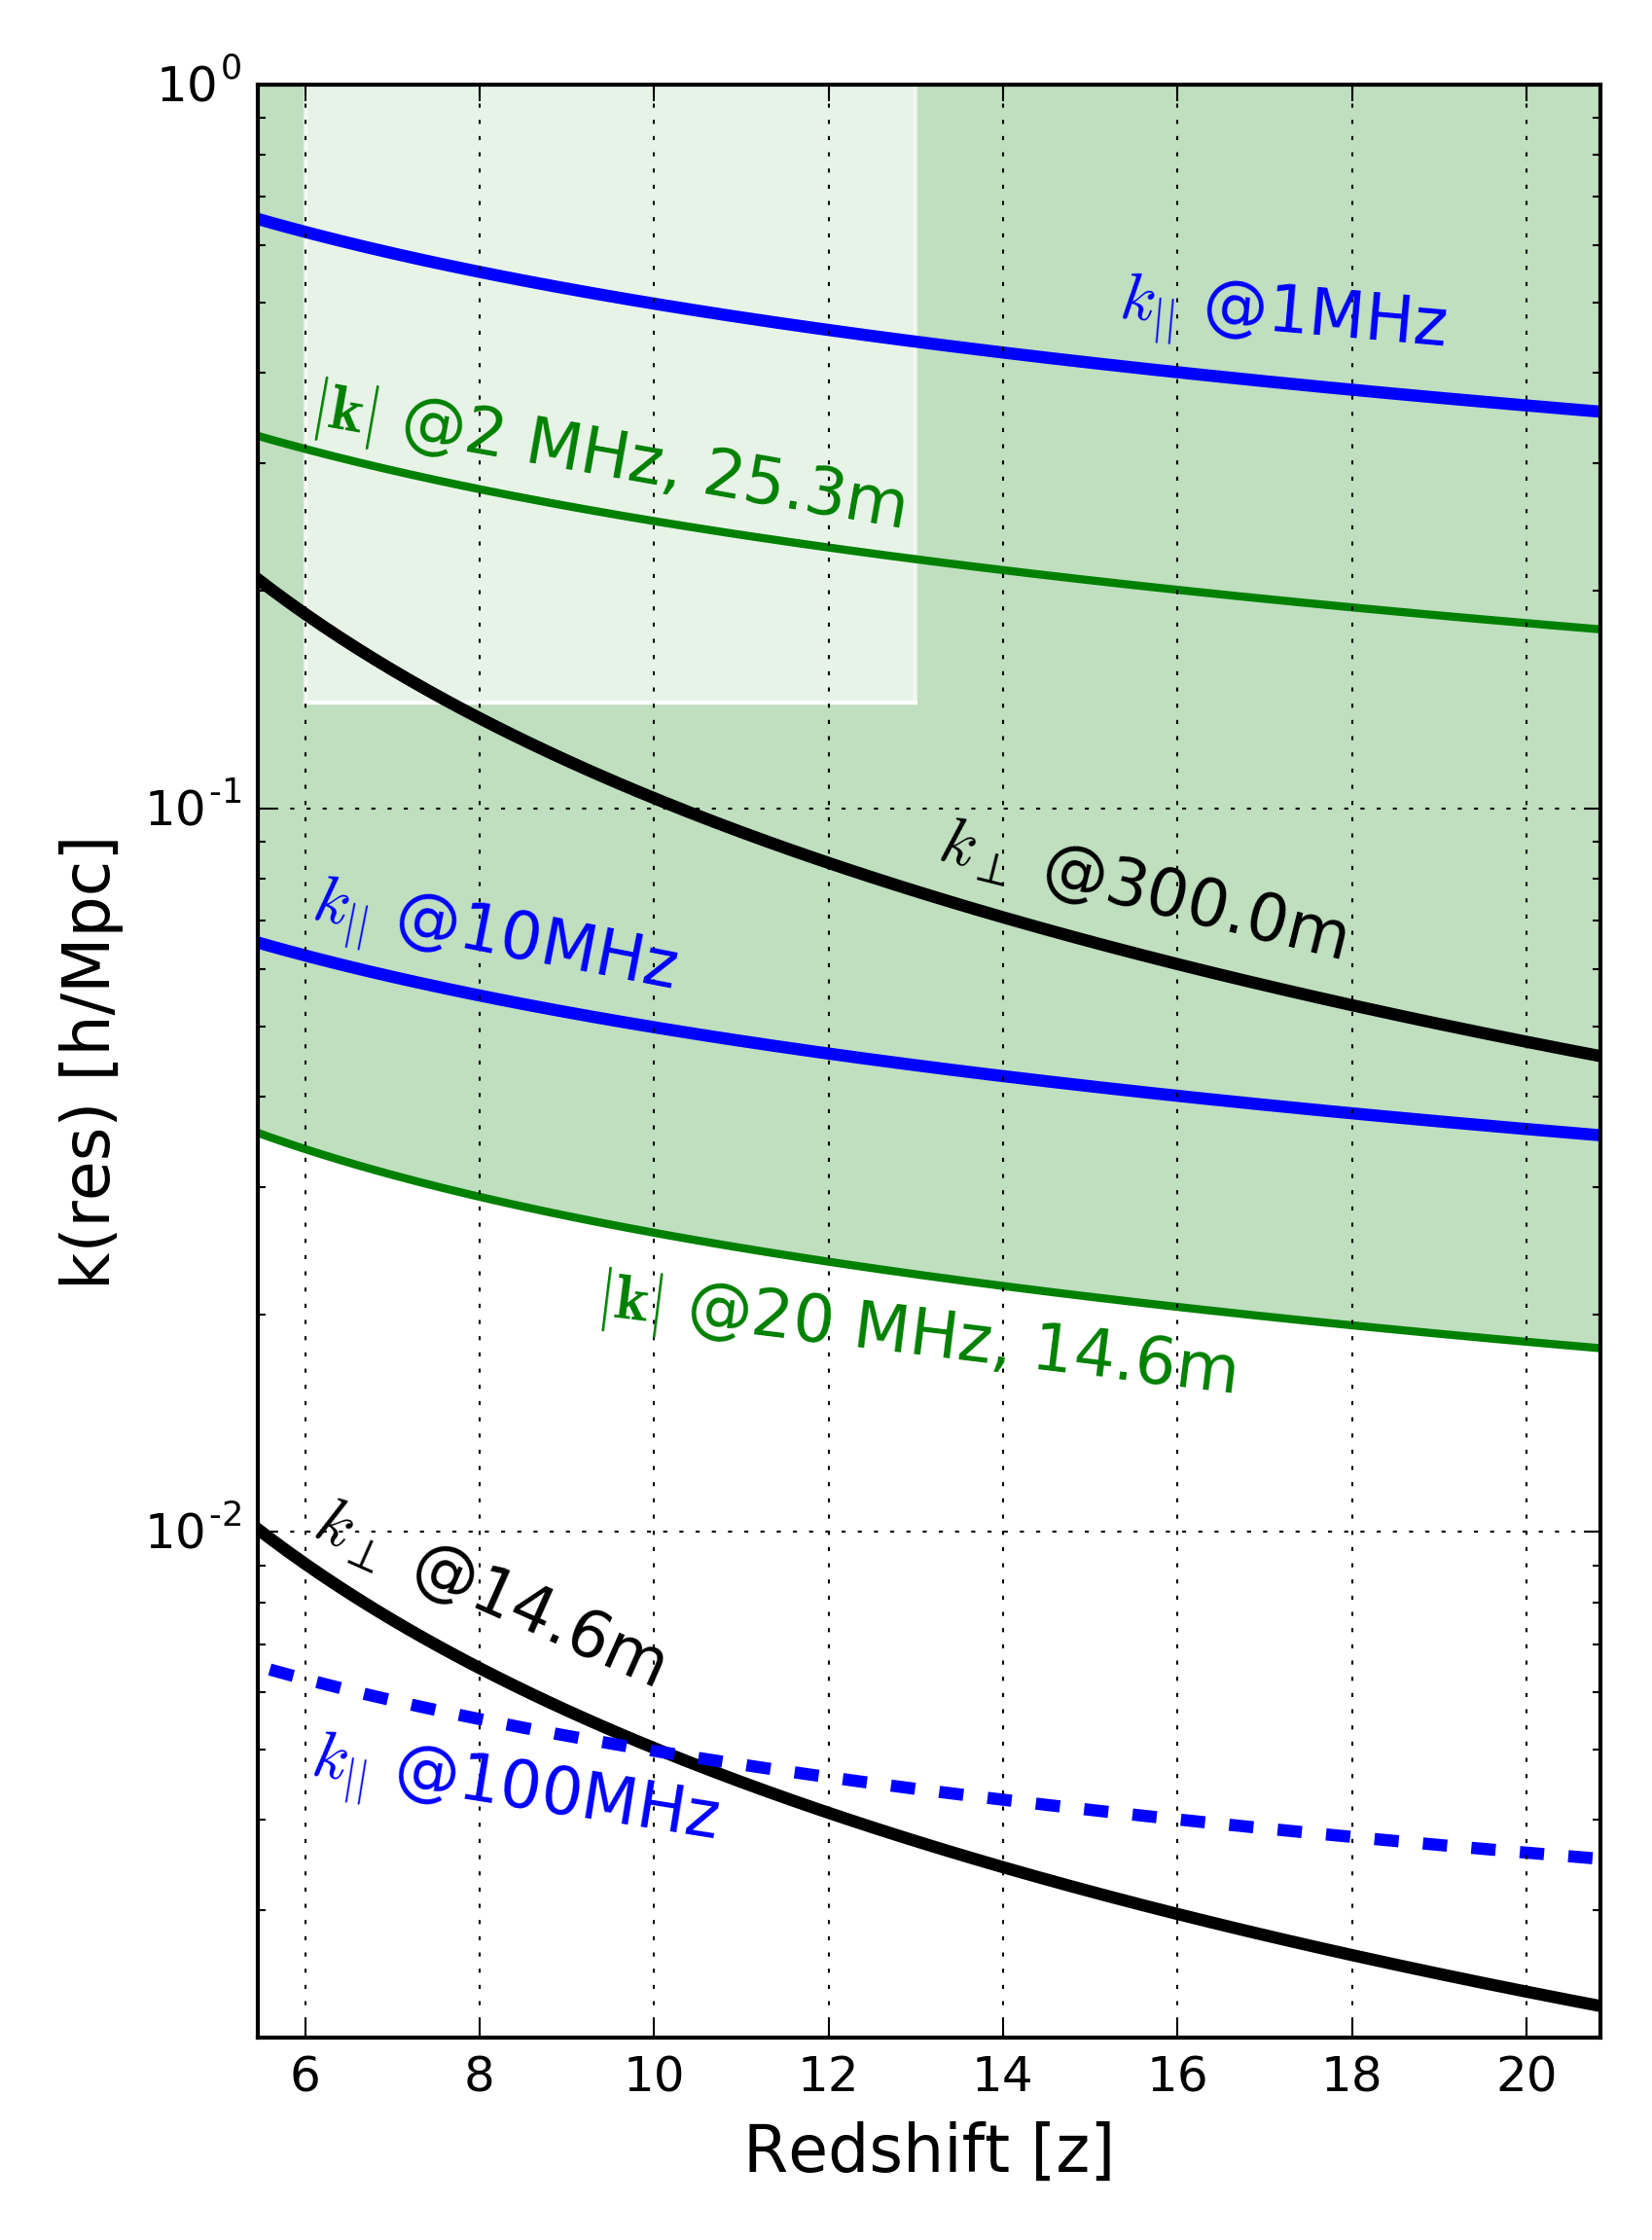
\includegraphics[width=.4\textwidth]{plots/kperf.png} 
}
\caption{\small kperf}
\label{fig:kperf}
\end{figure}

\subsection{Map-Making Approach}
\label{sec:mapapproach}
In contrast to the delay-spectrum approach, map-making approaches combine baselines to build up information before squaring and calculating the power spectrum.  The conceptually easiest approach is to first make an image cube of the sky as a function of angular position and frequency, and then to Fourier transform, square, and bin the cube to determine the power spectrum. One advantage of such an approach is that sky images can be interesting in their own right, both for dealing with measurement systematics and for accessing the non-Gaussian observational signatures (such as ionized bubble structures) that are missed by variance statistics such as the power spectrum. The principal disadvantage of a map-making approach is its stringent calibration and forward-modeling requirements for propagating models of bright foregrounds through instrument systematics. In contrast, the delay-spectrum allows one to stay considerably closer to the format of raw visibility measurements, thus allowing systematic effects to be sequestered to localized regions of parameter space where they can much more easily be filtered out.

\subsection{Hybrid Approaches}
\label{sec:hybridapproach}

While they were presented separately above, the delay-spectrum and map-making approaches need not be viewed as mutually exclusive. For example, mapmaking need not be limited to the real space image basis; pipelines that combine multiple baselines into estimates of various Fourier amplitudes of the sky are formally also mapmaking pipelines. Like the delay-spectrum approach, such pipelines (see, e.g., \citealt{trott_et_al2016}) avoid the image domain entirely. This helps to prevent artifacts that may introduced by imaging algorithms.

More generally, it is possible to express a map-making algorithm as a linear operator that acts on visibility data to produce a compressed dataset. Squaring this to obtain an estimate of the power spectrum then results in a weighted quadratic combination of visibilities, where one multiplies the visibility from every baseline with that from every other baseline. These visibility product pairs are subsequently normalized to form their own individual estimates of the power spectrum before all the normalized pairs are summed together to form a final power spectrum. Measuring a power spectrum in this way combines the best aspects of the mapmaking and delay-spectrum approaches. Power spectra are formed directly by the cross-multiplication of visibility data, preserving the delay-spectrum approach's strategy of staying close to quantities measured by an interferometer; on the other hand, by multiplying together the data from every possible combination of baselines, one retains all the information captured by mapmaking. Indeed, it can be shown \citep{liu_et_al2014a} that in the limit of infinitely fine Fourier space bins, the hybrid method that we have just described is mathematically equivalent to the mapmaking approach. In practice, the hybrid method comes with the added benefit of allowing particular baseline pairs that are suspected of being affected by instrumental systematics to be more surgically downweighted.

\subsection{Calibration}
\label{sec:calibration}



\section{High-Level Requirements} 
\label{sec:requirements}
From the science and techniques discussed above, we may derive some high-level requirements, predicating on optimizing for the delay-spectrum approach for detecting the EOR while not unduly limiting other approaches or other science goals.  The fact that HERA is an experiment and not meant to be a long-term general use facility greatly facilitates this optimization. This section describes the element, configuration, frequency and sensitivity requirements that largely set the overall design concept.

\subsection{Antenna Design and Configuration}
Thus, to open the widest possible window for EoR measurements, HERA must use close-packed antennas that
minimize signal reflections and deliver significant forward gain relative to their horizon response.
Tests with prototype HERA antennas (Figs. \ref{fig:orbcommexptandbeammap} and \ref{fig:reflectometry}, discussed in \S\ref{sec:antenna})
indicate that a moderately large parabolic dish with a short focal height can meet these requirements
\citep{ewall-wice_et_al2016-EoXLimits,neben_et_al2016,thyagarajan_et_al2016}.


\subsection{Frequency and Bandwidth}
Figure \ref{fig:cosmos} indicates the frequency range requirement to probe the expected timescale of the epoch of reionization using the 21cm line of hydrogen as the probe.  
These limits are derived from to-date complementary probes of reionization which include measurements of
the optical depth to last scattering in the CMB, QSO spectra, Ly-$\alpha$
absorption in the spectra of quasars and gamma ray bursts and the demographics
of Ly-$\alpha$ emitting galaxies
(Figure~\ref{fig:IonHist}). 
Constraints from these probes are still weak:
Ly-$\alpha$ absorption saturates at very small neutral fractions; galaxy
surveys directly constrain only the bright end of the luminosity function and
depend on an unknown escape fraction of ionizing photons to constrain
reionization; CMB measurements probe an integral quantity subject
to large degeneracies. Even when these observations are
combined into a single 95\% confidence region, the bounds remain weak.
For example, $x_{HI}$ spans almost the entire allowable range of [0,1]
at $z=8$. 21\,cm reionization experiments place much tighter constraints on ionization, with the
red band showing the forecasted 95\% confidence region derived from HERA data,
after marginalizing over astrophysical and cosmological parameters.


From these measurements and models, HERA is required to cover a redshift range of $z=$6 to 13, corresponding to a frequency range of 101 - 203 MHz.  We adopt 100-200 MHz for full performance as the requirement.  Extending the science to include the Dark Ages remains a goal so that efforts are on-going to design a feed to increase the lower limit down to at least 70 MHz without compromising the performance in the above requirement range.  The fall-back position for the low-frequencies is a serial deployment of a scaled version of the HERA feed or to potentially build additional elements specifically for the low-frequencies.  The 100 MHz bandwidth is also the minimum fully digitized and correlated bandwidth.

The scientific requirement on channel bandwidth is to allow access to k-modes of greater than 1 h/Mpc [ref], which requires about 256 channels over the 100 MHz bandwidth.  However, in order to handle radio frequency interference as well as to allow the bandpass to be characterized, a specification of 1024 channels has been chosen.  This yields a channel bandwidth of 97.7 kHz.

As mentioned earlier (see Fig. \ref{fig:kperf}) we should be able to process at least 10 MHz 

\begin{figure}[t]
\centerline{
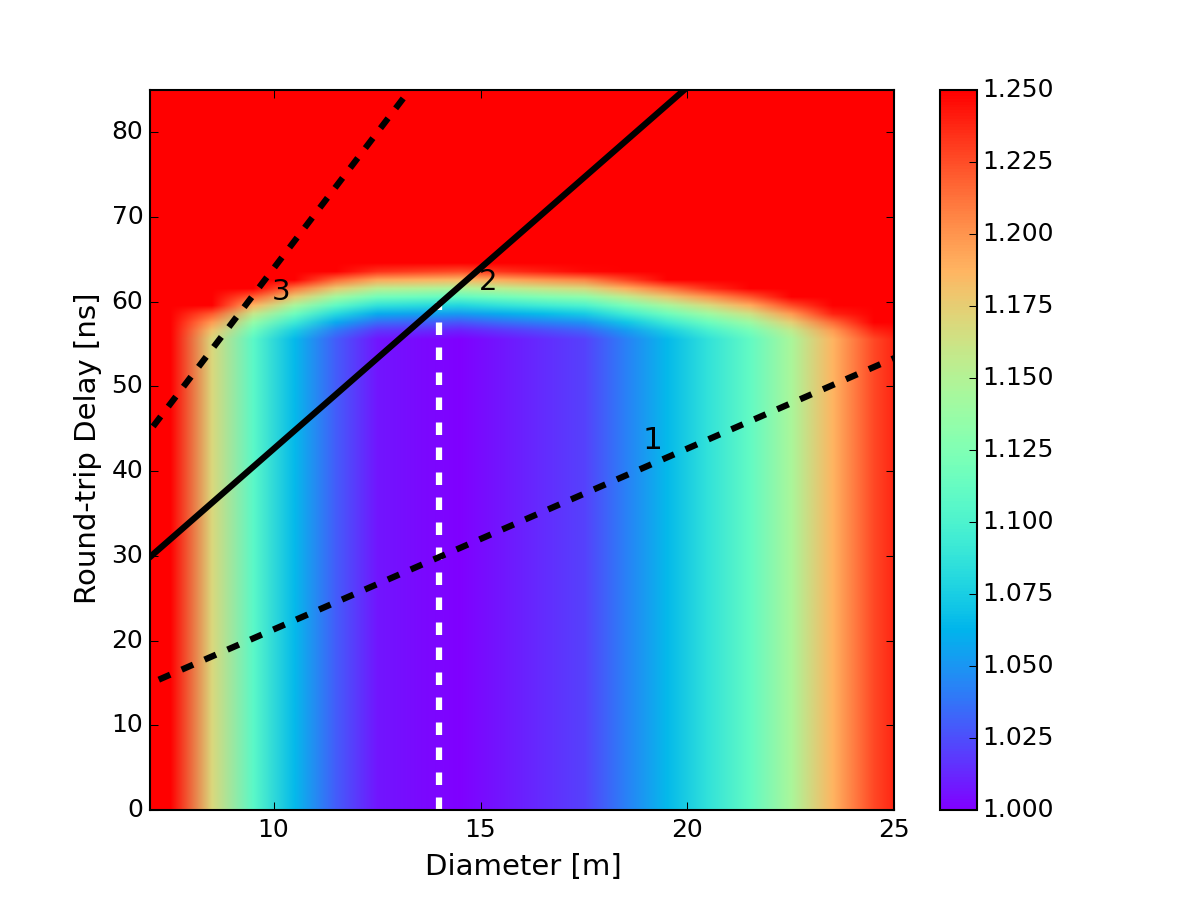
\includegraphics[width=7.5cm]{plots/costfigNew.png} 
}
\caption{\small Costing model for a fixed sensitivity system as a function of diameter (thick blue line and left axis) as well as the round-trip delay for 1,2 and 3 feed-vertex trips (dashed red lines and right axis).  The 60 ns spec is indicated by the horizontal dash line, and the two-trip intersection at about 14-meter is the vertical dashed line.  SEE TEXT...
\label{fig:costfig}}
\end{figure}



\subsection{Sensitivity Optimization}
\label{sec:cost}
As an instrument to characterize the power spectrum over its evolution, the specification on sensitivity is to make at least a nominal detection over the redshift region of support, or $z$=6-12, along with a very robust detection at the peak.  As seen in Fig. \ref{fig:Sensitivities} and Table \ref{tab:signif}.
To determine the optimal diameter, full system costings were done on a range of diameter sizes from 5m - 25m, where the total number was constrained to keep constant sensitivity for this measurement, which is shown in Figure \ref{fig:costfig}.  This included the full system, except the post-processing.  By assuming canonical values of 331 14-meter antennas, the number of elements needed for a given diameter to match the sensitivity is
\begin{equation}
N_a = 4634/D_a
\end{equation}
where $N_a$ and $D_a$ are the number of antennas and their diameter respectively.  Note that the number-diameter dependence was derived by running multiple sensitivity codes ({\em e.g.} Pober) over a range of values for the HERA configuration.  This dependency differs from Mellema, mostly likely due to the assumed configuration.
Figure \ref{fig:costfig} shows the resulting normalized system cost/performance-curve as the horizontal shading relative to the canonical HERA design 
which becomes very flat (colored purple) for diameters greater between about 12 and15 m, which is consistent with the chosen value of 14 meters based on other system considerations.


\section{System Design} \label{sec:design}

\noindent As described in the previous section, we have applied 
critical insights from first generation 21\,cm EoR experiments to define
the requirements for HERA---an instrument that ensures foregrounds remain bounded
within the wedge while \emph{delivering the sensitivity for
high-significance detections of the 21\,cm reionization power spectrum with
established foreground filtering techniques} 
\citep{pober_et_al2014,greig_and_mesinger2015}.
In this section, we summarize key features of the HERA design (see Table~\ref{tab:BasicParameters}) 
and system architecture (see Fig.~\ref{fig:overallBlockDiagram}).
This architecture
directly inherits from the PAPER and MWA experiments; HERA begins by reusing the
analog, digital, and real-time processing systems deployed for PAPER-128.  As HERA develops, this
architecture is incrementally upgraded to improve performance and add features while simultaneously
addressing issues of modularity and scalability.  As with PAPER, HERA proceeds in stages of development,
with annual observing campaigns driving a cycle of development, testing, system integration, calibration, and analysis.
This cycle ensures that HERA's instrument is always growing, that systematics are being found and eliminated at the
earliest build-out stages, that data analysis pipelines are tested and debugged while data volumes are smaller,
and that HERA is always producing high quality science.

\begin{table}[t]
\small
\begin{center}
\begin{tabular}{l | l}
\multicolumn{1}{c}{\emph{\textbf{Instrument Design Specification}}} & \multicolumn{1}{c}{\emph{\textbf{Observational Performance}}}\\
\hline
\textbf{Element Diameter:} 14\,m & \textbf{Field of View:} 9\arcdeg \\
\textbf{Minimium Baseline:} 14.6\,m & \textbf{Largest Scale:} 7.8\arcdeg\\
\textbf{Maximum Core Baseline:} 292\,m & \textbf{Core Synthesized Beam:} 25\arcmin\\
\textbf{Maximum Outrigger Baseline:} 876\,m & \textbf{Outrigger Synthesized Beam:} 11\arcmin\\
\textbf{Frequency Range:} 50--250\,MHz & \textbf{Redshift Range: $4.7 < z < 27.4$} \\
\textbf{Frequency Resolution:} 97.8\,kHz & \textbf{LoS Comoving Resolution:} $1.7$\,Mpc (at $z=8.5$)\\
\textbf{Survey Area:} $\sim 1440$ deg$^2$ & \textbf{Comoving Survey Volume:} $\sim 150$\,Gpc$^3$ \\
$\mathbf{T_\textbf{sys}}$: $100 + 120 (\nu/\rm{150~MHz})^{-2.55}$ K & \textbf{Sensitivity after 100\,hrs:} 50 $\mu \rm{Jy}~\rm{beam}^{-1}$  \\
\hline
\end{tabular}
\Caption{-0.1in}{0.99}{-0.4in}{HERA-350 design parameters and their observational consequences. Angular scales computed at 150\,MHz.}
\label{tab:BasicParameters}
\vspace{.2in}
\end{center}
\end{table}


\begin{figure}[h]
	\centering
	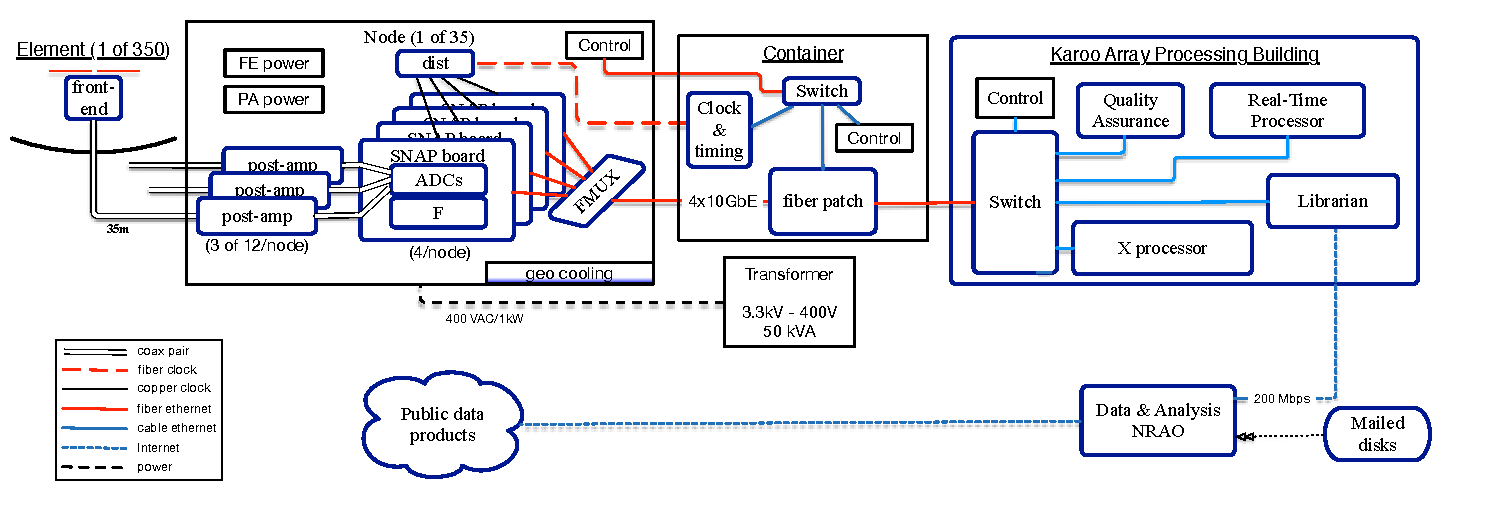
\includegraphics[width=1\textwidth]{plots/HERA_high_level_block_diagram.pdf}
	\caption{HERA's signal path.  Front-end amplifiers at the antenna feed drive signals on short coaxial cables to 
field nodes.  Nodes contain post-amplifiers and Smart Network ADC Processor (SNAP) boards that digitize, channelize,
and packetize data for optical transmission in 10 Gb Ethernet format.  Optical fibers are aggregated in a field container
onto a 10 km fiber bundle connecting to the Karoo Array Processing Building, where signals are cross-multiplied
in the X processor.  After correlation, visibilities are stored by the Librarian, compressed and redundantly calibrated
by the Real-Time Processor, and transmitted over the network to clusters for storage and analysis.  Final products are
hosted on public-facing NRAO servers, with a web interface for selecting and downloading data.}
	\label{fig:overallBlockDiagram}
	\vspace{-5pt}
\end{figure}

\subsection{Antenna Element}
\label{sec:antenna}
\vspace{-5pt}

As discussed in the previous section, the design of the design principles are three-fold:
\begin{itemize}
\item optimize for the delay-spectrum technique of measuring the EOR power spectrum,
\item minimize costs, and
\item the experiment has a limited lifetime of about five years.
\end{itemize}
The first item primarily means that chromatic effects corresponding to delays appropriate for the measurement described above must be below the expected signal level, which essentially determines the focal length.  The second item constrains the diameter and element count, as well as the focal length over diameter ratio ($f/D$), based on a cost function and maximizing sensitivity per element.  And the third items constrains the construction materials and methods and the operational model.  This led to a fixed transit element with a diameter of 14 meters.

The construction materials are readily available standard construction materials, making for a very cost-effective design.  The feed is supported from three utility poles using line and hardware primarily from boating activities which can handle the load and external environment.  Given the close-packed design, each pole (except for the perimeter) are shared between three antennas.  This both reduces the number of poles, but also makes for a balanced load.  Note that the perimeter poles can be stayed with guy lines if needed.  A close-up of one antenna is shown in Fig \ref{fig:elementpic}.  The rim is also supported off of these poles, with three smaller posts in between such that the outer perimeter is regular dodecagon shape.  

The center of the antenna is a cast concrete donut-shaped hub with 12 angled sleeves for PVC spars which provide the support for the surface and 12 horizontal spars which allow for additional support.  The twelve spars are made of 60mm PVC pipe, which are stressed along three support points to approximate a parabolic shape.  Note that an ideal moment-loaded beam actually attains a true parabola.  Note that the three support points (one at the hub, one about 3 meters out radially and one at the rim-end) are at the correct height and angle for the underlying parabola.  

The shape between the spars is actually a one-dimensional parabola rather than a two-dimensional paraboloid, so the dish surface may more properly be called a ``facetted parabola''.  If only twelve spars were used for the entire surface, simple Ruze losses would be quite high (about 10\% at 150 MHz).  Therefore, at about 2.1 meters another horizontal member is placed, which launches another parabolic spar.  The simple Ruze loss is then less than 1\%, which is much more acceptable.  Fig \ref{fig:elementplan} shows this surface scheme and the panelization (left) and the offsets (in mm) of that scheme from an ideal parabola.  The panel that is ``left out'' is the location of a door to allow access into the hub (via a small removable bridge).  The additional intermediate spars also make the panel sizes much more manageable and better secured.  The panel arrangement is also set by a standard width of mesh roll of 1.22m.

\begin{figure}[h!]
\centerline{
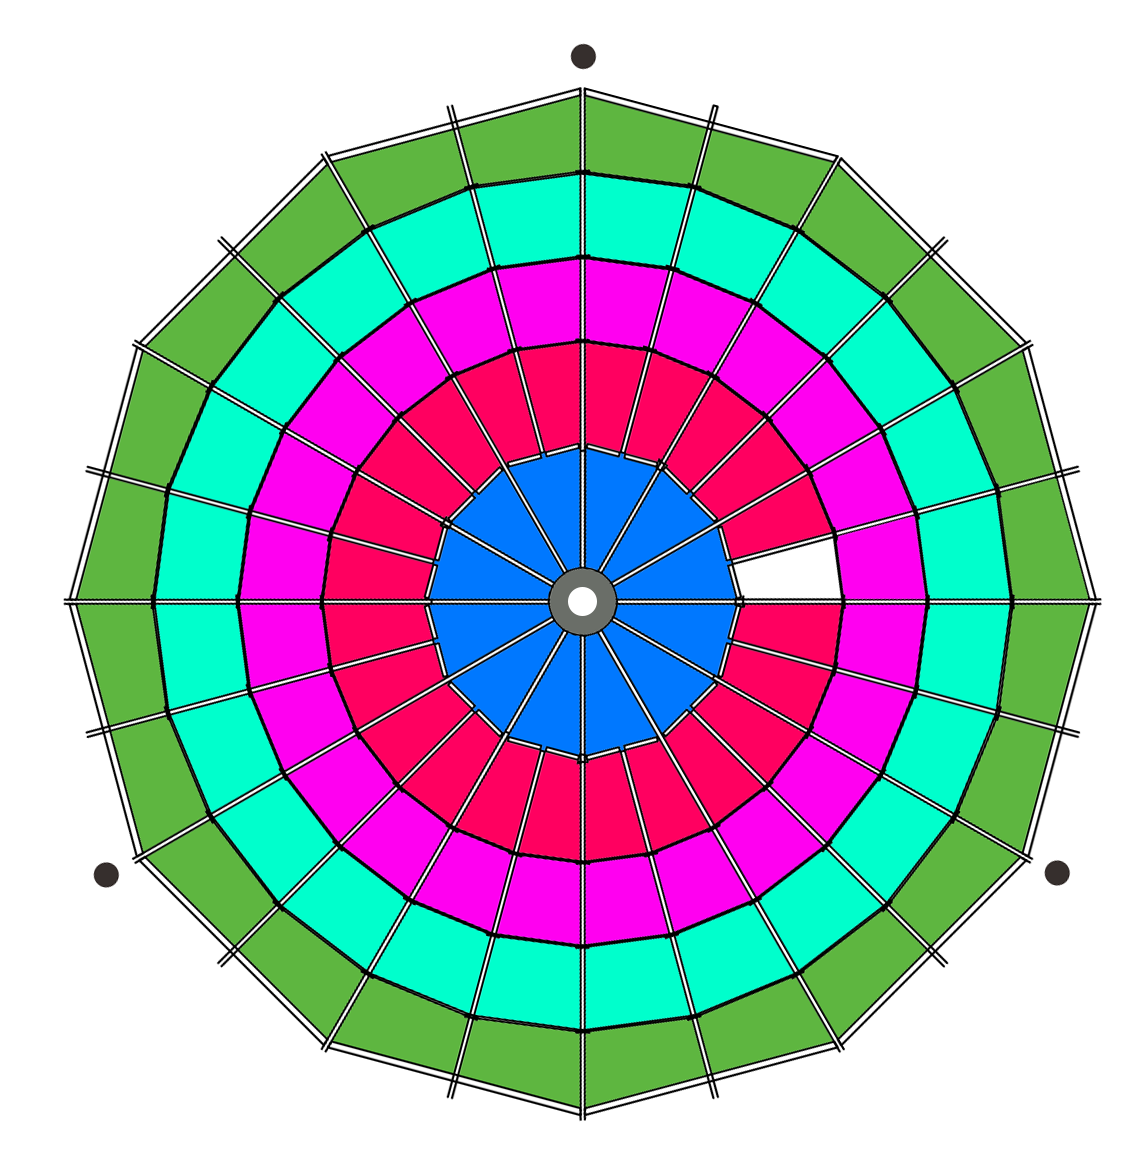
\includegraphics[height=6cm]{plots/antPlan.png}
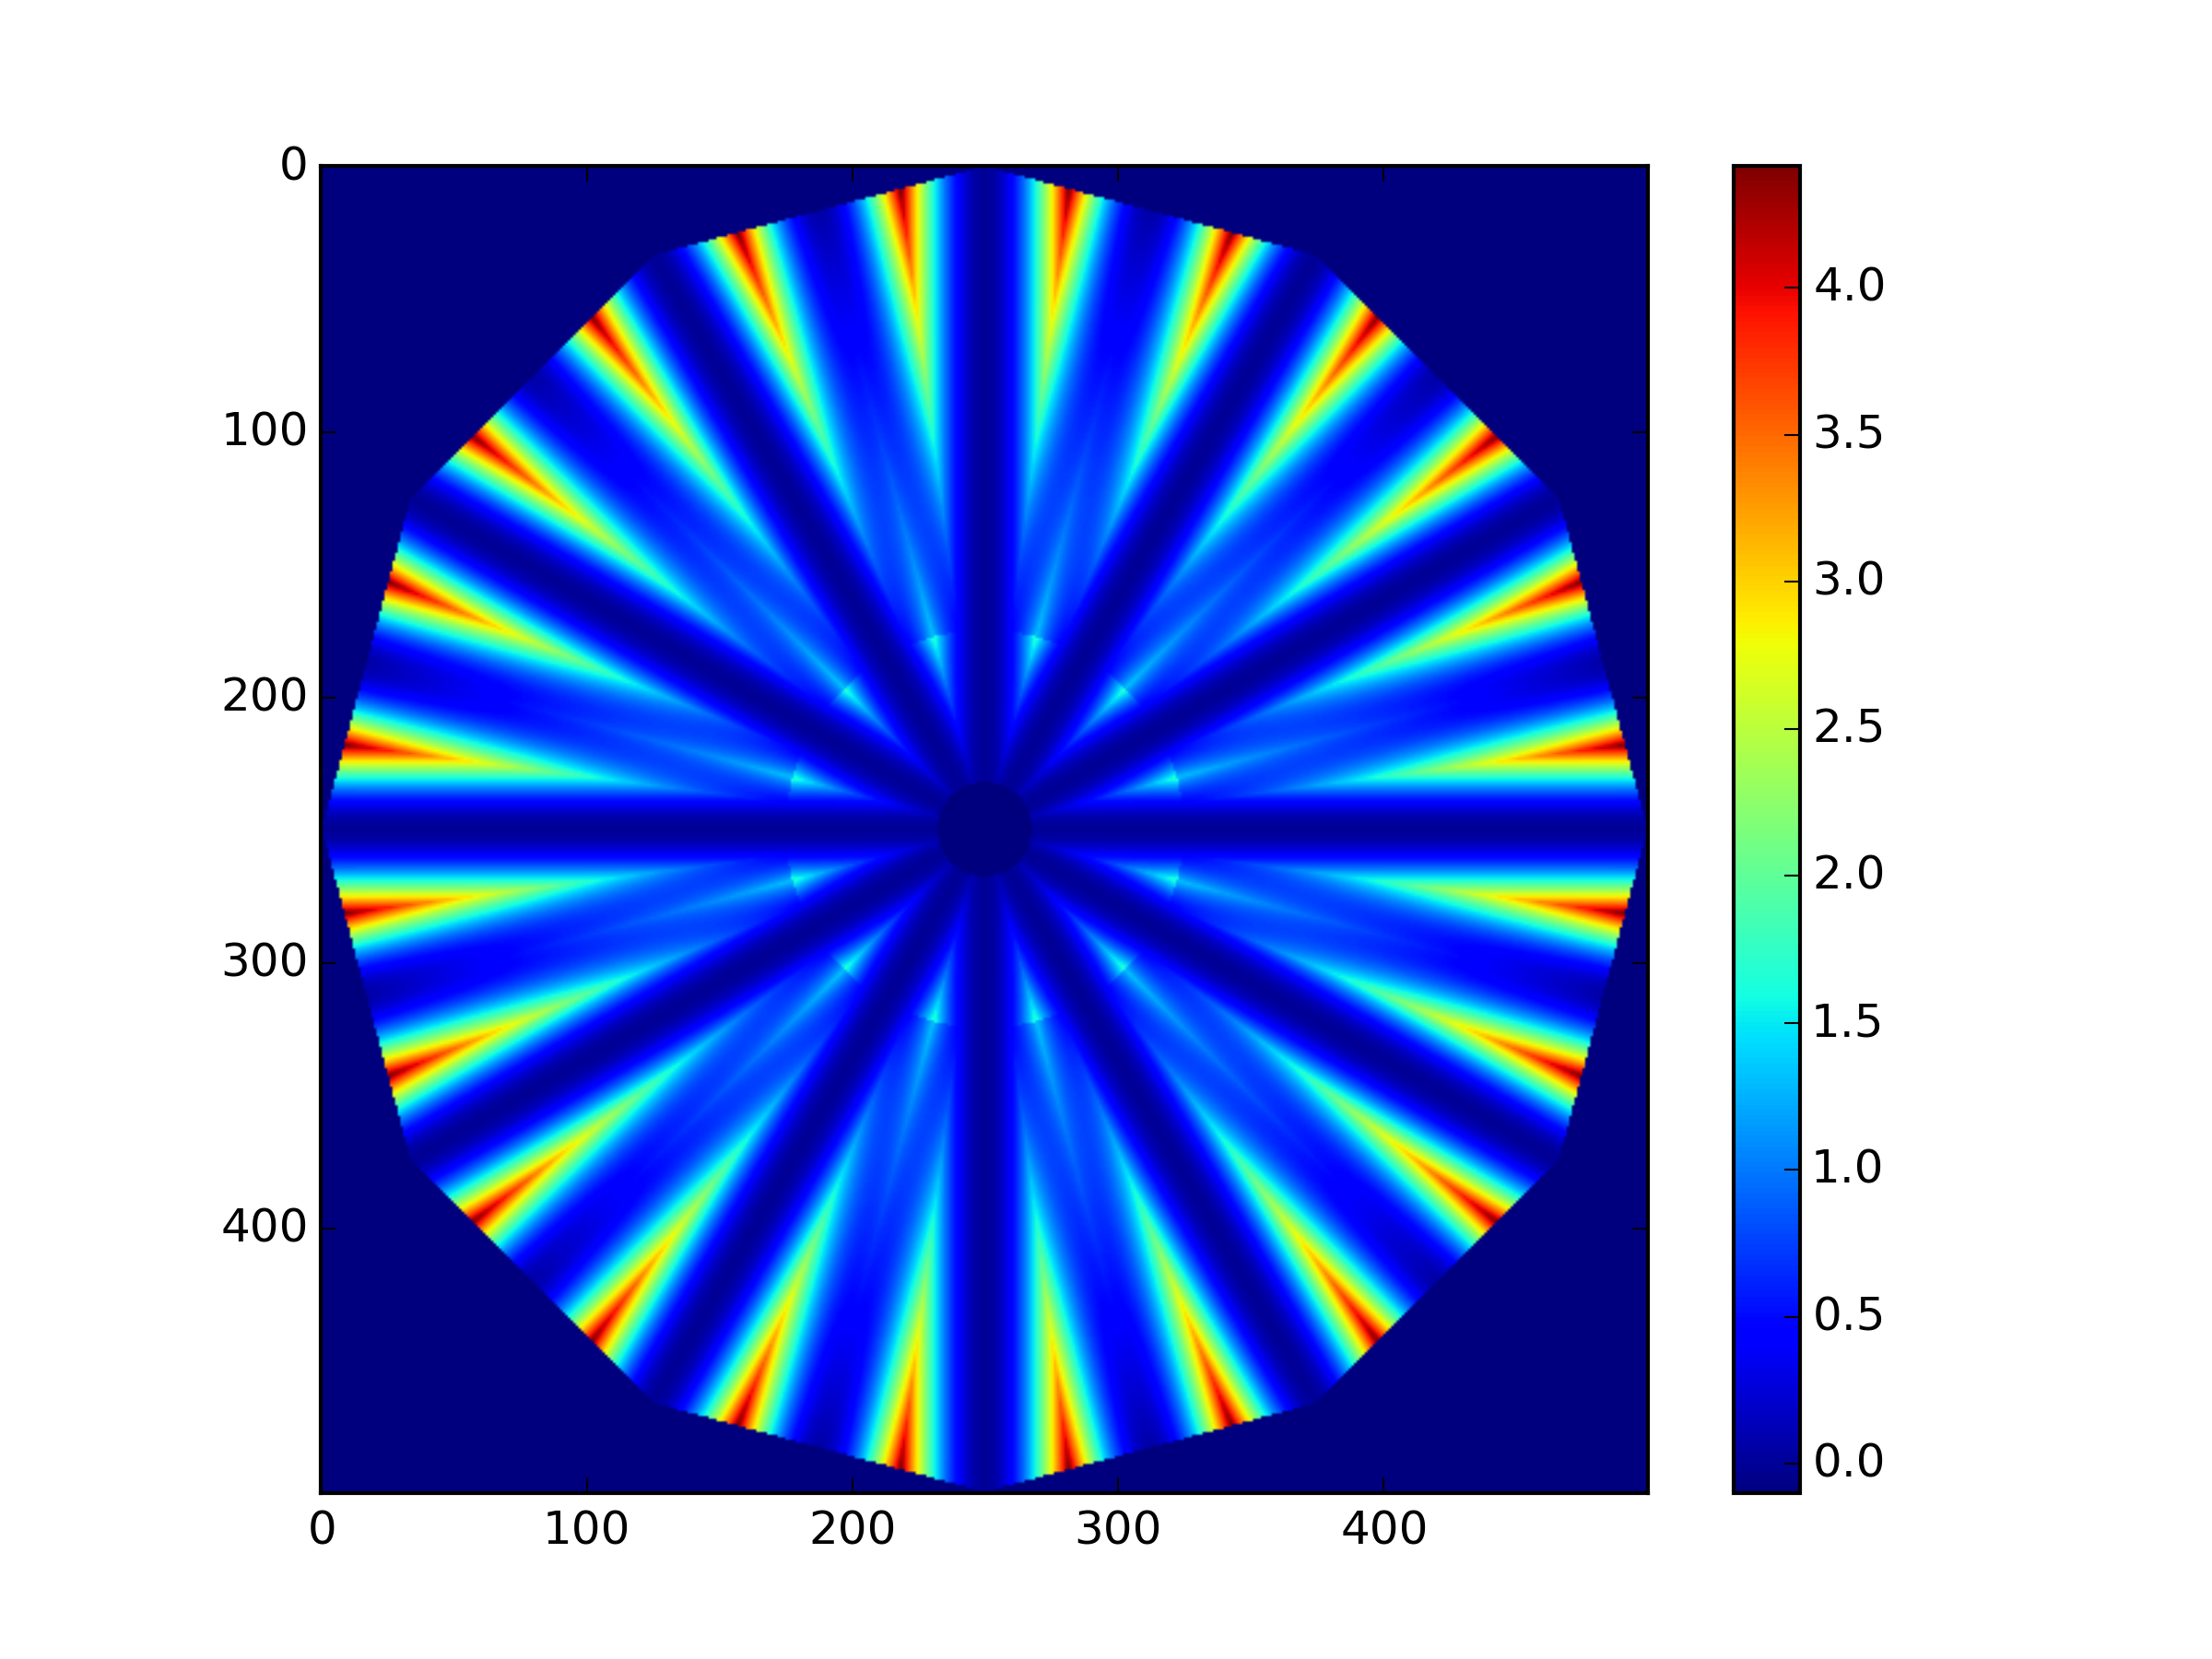
\includegraphics[height=6cm]{plots/offset.png} 
}
\caption{\small Element.
\label{fig:elementplan}}
\end{figure}

The feed is to be deployed along the two separate phases.  Initially, the feed reuses the dipole portion of the PAPER element, however in a new optimized cylindrical feed-cage configuration.  The optimization was based on main beam efficiency, cross-coupling (integrated feed pattern on dish), standing waves (blockage, {\em e.g.} Baars), and frequency response.  The design parameters were size of backplane, height of mast, height of skirt, and cone versus cylinder.  Cones were ruled out since it was found they introduce additional frequency structure with no real improvement in performance and a range of cylinders were evaluated.  The phase 1 design is documented in a memo \cite{feedmemo}, while additional studies are on-going at NRAO, University of Cambridge and Stellenbosch University.  The chosen feed design is shown in Figure X.

Additionally, to lessen cross-coupling, a screen fence around the perimeter is also under investigation.  Rather than being vertical, it will have a slight angle and potentially some edge treatment to try and lessen diffraction.  Tests of the antennas are discussed in a number of papers CITE.  Figure Y shows beam patterns.

As mentioned, the feed is supported by lines from the three poles via a rigid support to which the feed cage and dipole attach.  Another line goes down centrally to the hub to hold the feed rigidly in place at the correct height.

The low noise amplifier/balun integrates directly to the base of the feed dipole in the same configuration as per PAPER (REF).  The 150m length of 75 $\Omega$ cable also runs down centrally and then over to the post-amplifier module, which is housed near the RFI-shielded container containing the digital electronics.



\noindent The novel design of HERA's antenna element (Figs. \ref{fig:HERApictures} and \ref{fig:orbcommexptandbeammap}), now extensively field-tested with MSIP seed funding, 
is one of the critical advances that enables HERA to achieve its science
goals cost-effectively.  The 14-m fixed zenith-pointing parabolic dish strikes an optimal
balance between sensitivity and systematics.  The large collecting area of a
HERA element yields nearly 5 times the sensitivity of an MWA tile and more
than 20 times that of a PAPER element, but it does so without substantially
degrading our ability to isolate and remove foreground emission on the basis of
spectral smoothness (Fig. \ref{fig:reflectometry}, right panel).  As shown in
\Mycitet{parsons_et_al2012b}, the amplitude and timescale of signal reflections
relates directly to the leakage of smooth-spectrum foregrounds into regions of Fourier space 
used to measure reionization.
To facilitate foreground filtering, HERA's antenna element is designed to suppress reflections at long time delays.

\begin{figure}[h!]
	\begin{tabular}{ll}
	\begin{minipage}{4.2in}
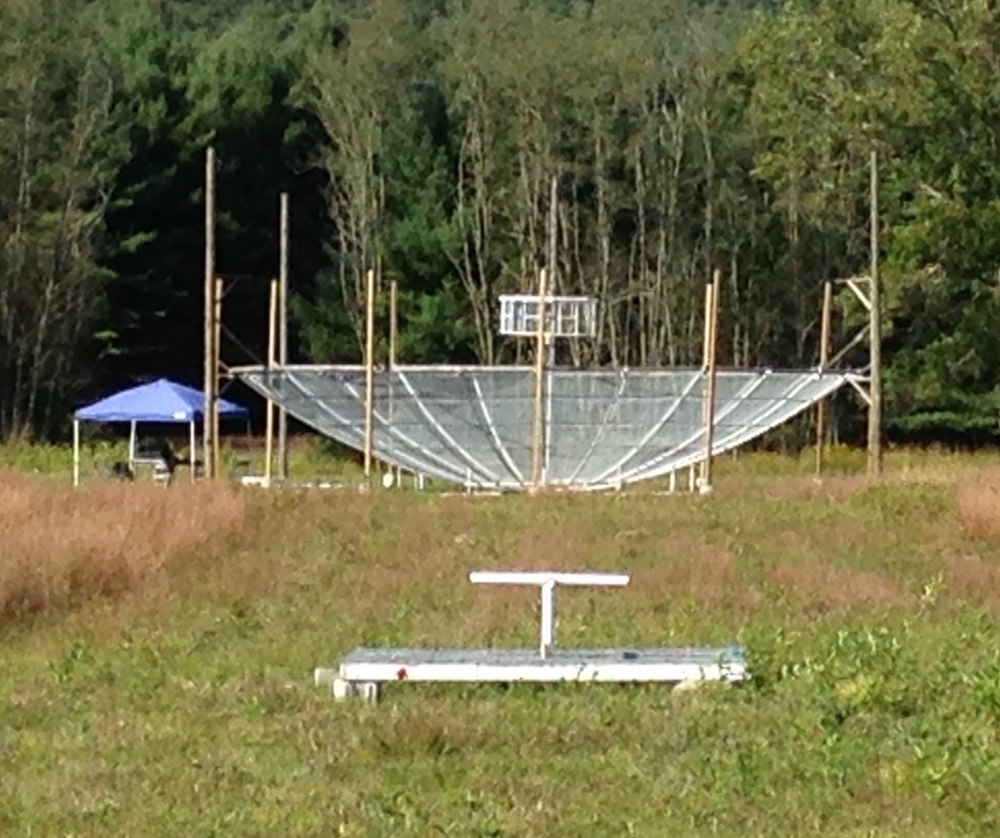
\includegraphics[width=2.1in]{plots/ref_dipole_and_hera_dish.jpg}
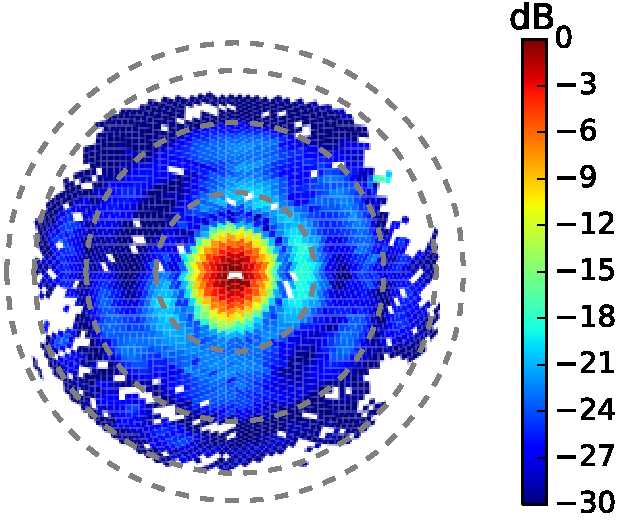
\includegraphics[width=2.1in]{plots/orbcomm_dish_beam_map_530cm_feed.pdf}
	\end{minipage} & 
	\begin{minipage}{2.05in}
	\caption{Left: The first of three prototype dishes at NRAO--Green Bank, used for measuring beam frequency structure with reflectometry and the beam pattern at 137\,MHz by comparing satellite signals to the reference dipole in the foreground \citep{neben_et_al2016}. Right: The measured EW power pattern plotted with dashed lines marking zenith angles of 20$^\circ$, 40$^\circ$, 60$^\circ$, 80$^\circ$.} 
	\label{fig:orbcommexptandbeammap}
	\end{minipage}
	\end{tabular}
	\vspace{-15pt}
\end{figure}

\begin{figure}[h!]
	\centering
    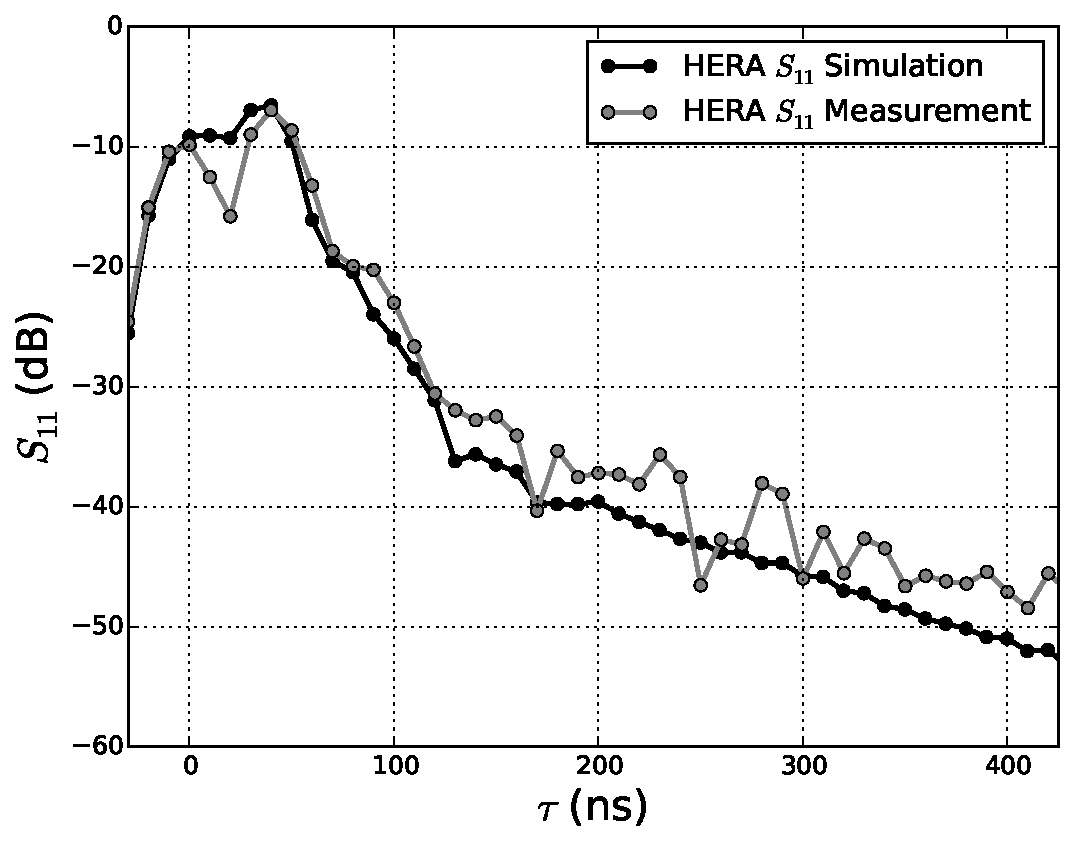
\includegraphics[width=0.49\textwidth]{plots/s11_compare_msip.pdf}
	%\includegraphics[width=0.49\textwidth]{plots/compare_kernels_msip_subband.pdf}
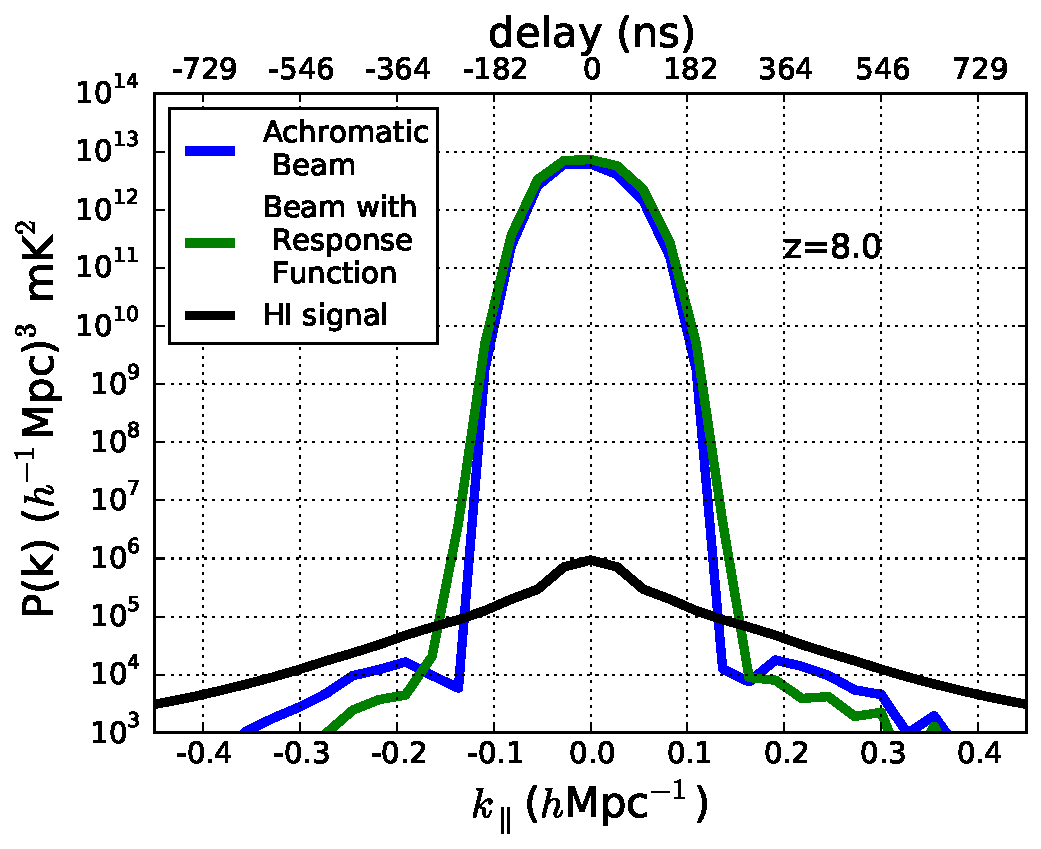
\includegraphics[width=0.5\textwidth]{plots/ps1d_with_delay_kernel.pdf}
	\vspace{-25pt}
	\caption{Left: Electromagnetic simulations (black; \citealt{ewallwice_et_al2016}) of the response of the HERA dish as a function of time delay, $\tau$,
       agree with field measurements (grey; \citealt{patra_et_al2016}). 
Right: Modeled foreground power spectra with (green) and without (blue) the antenna chromaticism over a 10\,MHz subband centered at $z=7.5$. The spectral smoothness of the dish enables foreground isolation below the level of a fiducial reionization signal (black) for most $k_{\parallel}$ modes, yielding percent-level constraints on model parameters.}
	\label{fig:reflectometry}
	\vspace{-10pt}
\end{figure}

As shown in Fig.~\ref{fig:reflectometry}, HERA's element meets this requirement in
reflectometry tests, performing comparably to the PAPER element.  The
relatively short (4.5\,m) focal height of the parabolic dish 
minimizes the timescale of feed-dish reflections while maintaining the feed's
illumination of the dish.  HERA's feed design is based on the PAPER sleeved
dipole element, inverted above a backplane, with a skirting cylinder to
improve symmetry in the polarized beam response patterns.  Figure
\ref{fig:orbcommexptandbeammap} shows the beam pattern measured at 137 MHz with a beam mapping
system using the ORBCOMM satellite network \Mycitep{neben_et_al2016}.  Results
indicate an effective per-element collecting area of 93\,m$^2$, compared with the
theoretical maximum Airy response of 155 m$^2$.  The measured primary beam is
consistent with simulations at the 0.1\% to 0.5\% level, with a full width at
half maximum of $\sim$$10^\circ$, and a first sidelobe at -20 dB \citep{ewallwice_et_al2016,neben_et_al2016,patra_et_al2016,thyagarajan_et_al2016}.
Feed-to-feed coupling between adjacent antennas has been measured to be below -50 dB, indicating
that mutual coupling will not be problematic.

With observing wavelengths of 1.5 to 3 m, meeting the required accuracy
in placing the components of HERA's dish is straightforward.
Dish centers are fixed
by a concrete hub placed with final surveyed accuracy of $\sim$10 cm.  These
hubs constrain radial PVC spars, tensioned into approximate parabolas against a
rim supported by utility poles.  The resulting faceted paraboloid has
a measured RMS surface accuracy of 3 cm, which is well within the 0.1$\lambda$ tolerance for
coherent phasing.  Feed placement relative to the dish is the most stringent requirement, with
a tolerance of 5 cm.  This placement is ensured by spring-tensioned Kevlar lines attached to
three utility poles at the dish rim and a 165-lb tensioning down to the concrete hub with
a fixed length line that ensures a correct focal height.  With 19 dishes constructed in South Africa
and 2 in Green Bank, we are confident in the ability of our trained field teams to construct HERA
elements to specification.


\subsection{Array Configuration}
\label{sec:arrayConfig}

\noindent HERA's 320 core elements are arranged in a compact hexagonal grid, split into three displaced segments 
to cover the $uv$-plane with sub-element sampling density (see Fig.~\ref{fig:arrayConfig}). The dense core maximizes 
sensitivity on the short baselines for which PAPER's proven foreground filtering strategy works best.
The core is supplemented by 30 additional outrigger elements 
to tile the $uv$-plane with instantaneously complete sub-aperture 
sampling out to 250$\lambda$ and complete aperture-scale sampling out to 350$\lambda$ (at 150\,MHz). This sampling 
strategy suppresses grating lobes in the synthesized beam and provides information for calibrating and correcting 
direction-dependent antenna responses \citep{dillon_parsons2016}.
Even with the sub-aperture dithering and long baselines, all 350 HERA elements can be robustly calibrated by taking advantage of 
its highly redundant configuration \citep{liu_et_al2010,zheng_et_al2014}. 
Resulting calibration errors range from $\sim5\%$ (in the core) to $\sim10\%$ (for outriggers)
of the residual fractional noise per antenna after averaging.

\begin{figure}[h]
	\centering
	\vspace{-5pt}
	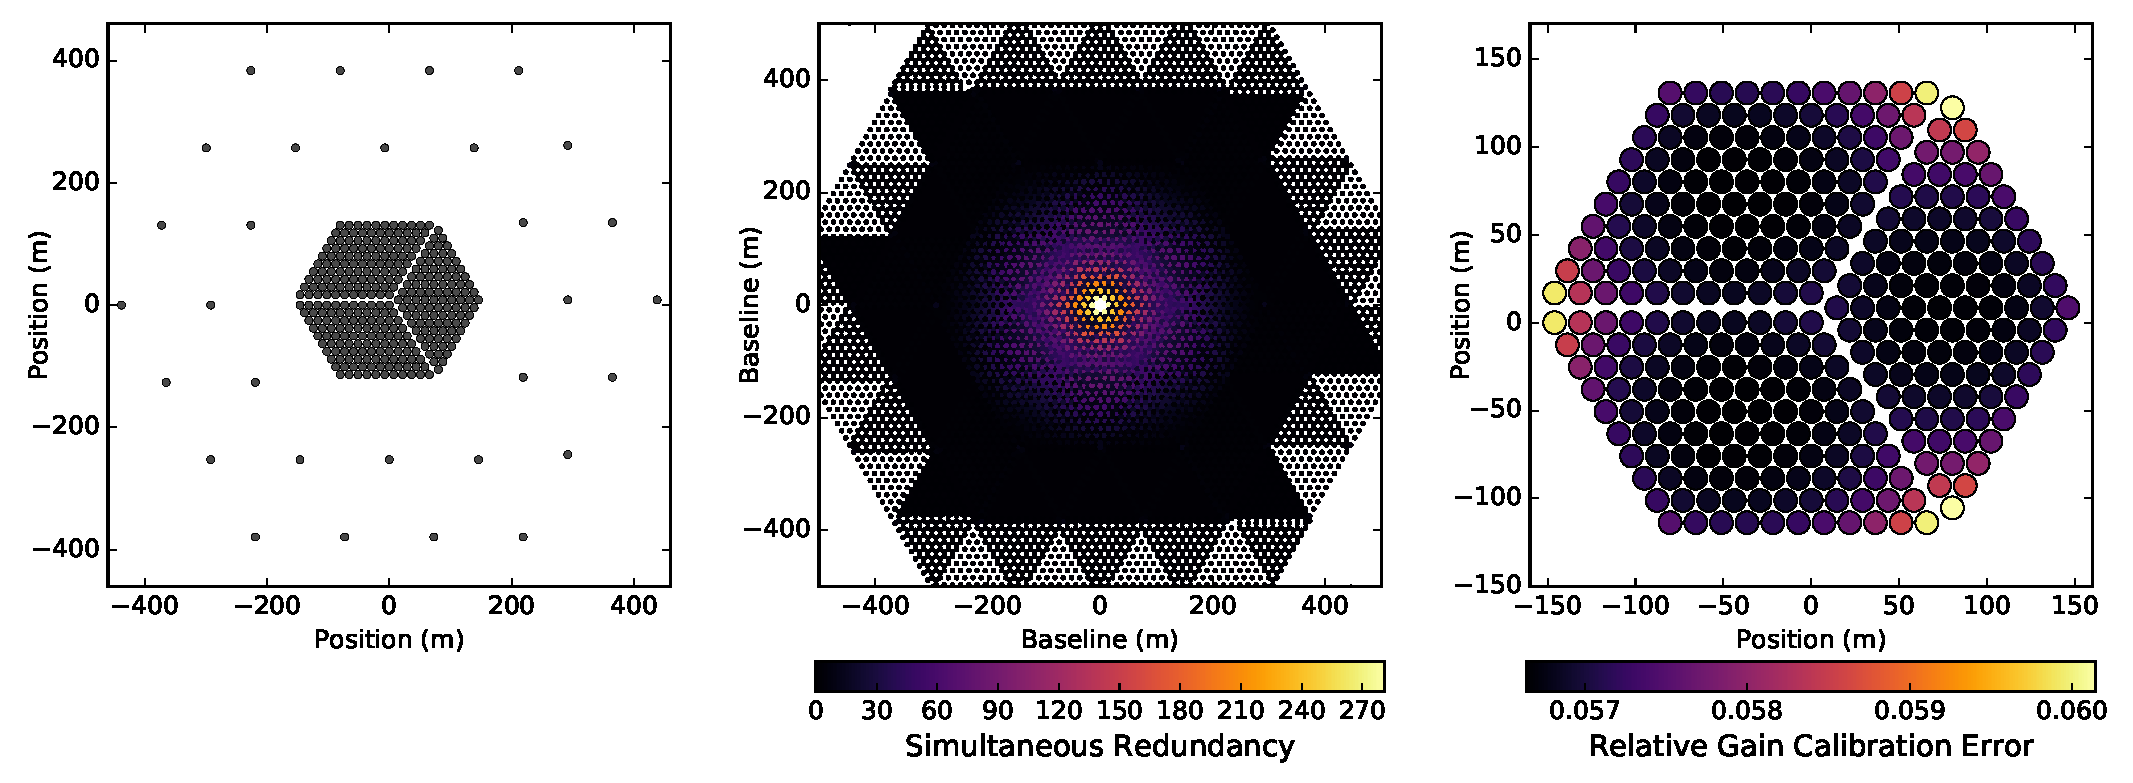
\includegraphics[width=1\textwidth,clip]{plots/HERA_Array_Config.eps}
	\vspace{-25pt}
	\caption{HERA's elements are divided between a 320-element, hexagonally-packed core and 30 outriggers (left). This produces instantaneous
$uv$ coverage at triple the element spacing out to 250$\lambda$ at 150\,MHz (middle). All 350 elements can be redundantly calibrated 
using the \citet{liu_et_al2010} technique, yielding calibration errors that are a small fraction of the residual noise per antenna (right).}
		\label{fig:arrayConfig}
			\vspace{-10pt}
\end{figure}

\subsection{Analog Signal Path}

\noindent HERA's analog signal path, which operates from 50--250 MHz, emphasizes spectral smoothness and robustness.
With receiver temperatures of 50--100 K readily achievable with ambient temperature electronics, 
sky noise dominates the system temperature of telescopes operating below 300 MHz.  As a result,
HERA's low-noise amplifiers (LNAs) are inexpensive, passively cooled components integrated into the
antenna feed.  
HERA's signal path emphasizes careful impedance matching between each component to avoid signal reflections that can induce foreground leakage.
In particular, impedance matching between free space (377$\Omega$) and coaxial cable (50$\Omega$) is undertaken
in the feed/balun at the front end of the signal chain, where the time constants of inevitable reflections are
minimized.  For a similar reason, HERA houses analog-to-digital converters (ADCs) in nodes near the antenna elements
to limit the total analog path length.

While building to 128 elements during the first two project years, HERA reuses PAPER's tested and characterized 
LNAs, cables, and post-amplifier modules, operating
from 100--200 MHz.  In the third project year, these components are replaced by the 50--250 MHz, length-constrained signal
path described above, supporting HERA's pre-reionization science and extending the lever-arm for modeling and suppressing smooth-spectrum foreground emission.

\subsection{Digital Signal Path}
\label{sec:digital}

\noindent Although correlator development has historically been one of the most 
expensive aspects of building a large radio interferometer, this is no longer the case.
CASPER \Mycitep{parsons_et_al2006}
open-sourced the development of digital signal processing engines for astronomy and
now has world-wide participation,
with over 500 members at 73 institutions, and 
five generations of hardware.
On a modest budget, PAPER applied CASPER technology to develop and deploy new correlators
annually for five years running, each quadrupling the computational capacity of its predecessor.
Led at UC Berkeley's Radio Astronomy Lab (RAL),
HERA efforts continue this incremental development cycle, using a packet-switched
correlator architecture \Mycitep{parsons_et_al2008} that both PAPER and LEDA have
applied to systems employing FPGAs and GPUs \citep{clark_et_al2011}.



In order to meet the 35\,m specification for a maximum analog signal path, along with a growing need for system scalability, HERA beyond the first 128 elements will adopt a node-based architecture for amplification, digitization, channelization, and digital
transmission in the field, building on MWA heritage. This design is merged with PAPER's clean 
architecture for real-sampling and channelizing the entire analog passband at once, packetizing the data into
10 Gb Ethernet format, and relying on commercial switches to perform the frequency/antenna corner-turn required for FX correlators

{\bf Node}. HERA-350 employs RFI-tight node enclosures that each contain the final gain and digitization stages for
signals from 12 antennas, along with power supplies, cooling, sensors, and a small server for monitor/control.  
As part of previous HERA support,
a new Smart Network ADC Processor (SNAP; Fig.~\ref{fig:hardware}) board has been incorporated 
into the Collaboration for Astronomy Signal Processing and Electronics Research (CASPER) suite of hardware and firmware. This inexpensive board was co-designed by UC Berkeley and NRAO to be
both the digitizer and F-engine in HERA's FX correlator architecture.
Each SNAP board 
digitizes and channelizes a 0--250 MHz band for 6 input signals (3 antennas, dual-polarization).
A 200-MHz band of selectable channels is transmitted over optical fiber
to a central container (see below), and on to the correlator.  Laboratory
tests have successfully demonstrated robust transmission from the SNAP board, through 10 km of fiber optic cable, 
into a 10 GbE switch using inexpensive, commercially available optical transceivers.
Activities under this proposal include 
testing and extending FPGA firmware,
integrating and testing all components in the node subsystem, and providing a monitor/control
access interface.

\begin{figure}[h]
\centering
%\includegraphics[width=2.2in]{plots/ROACH2.png}
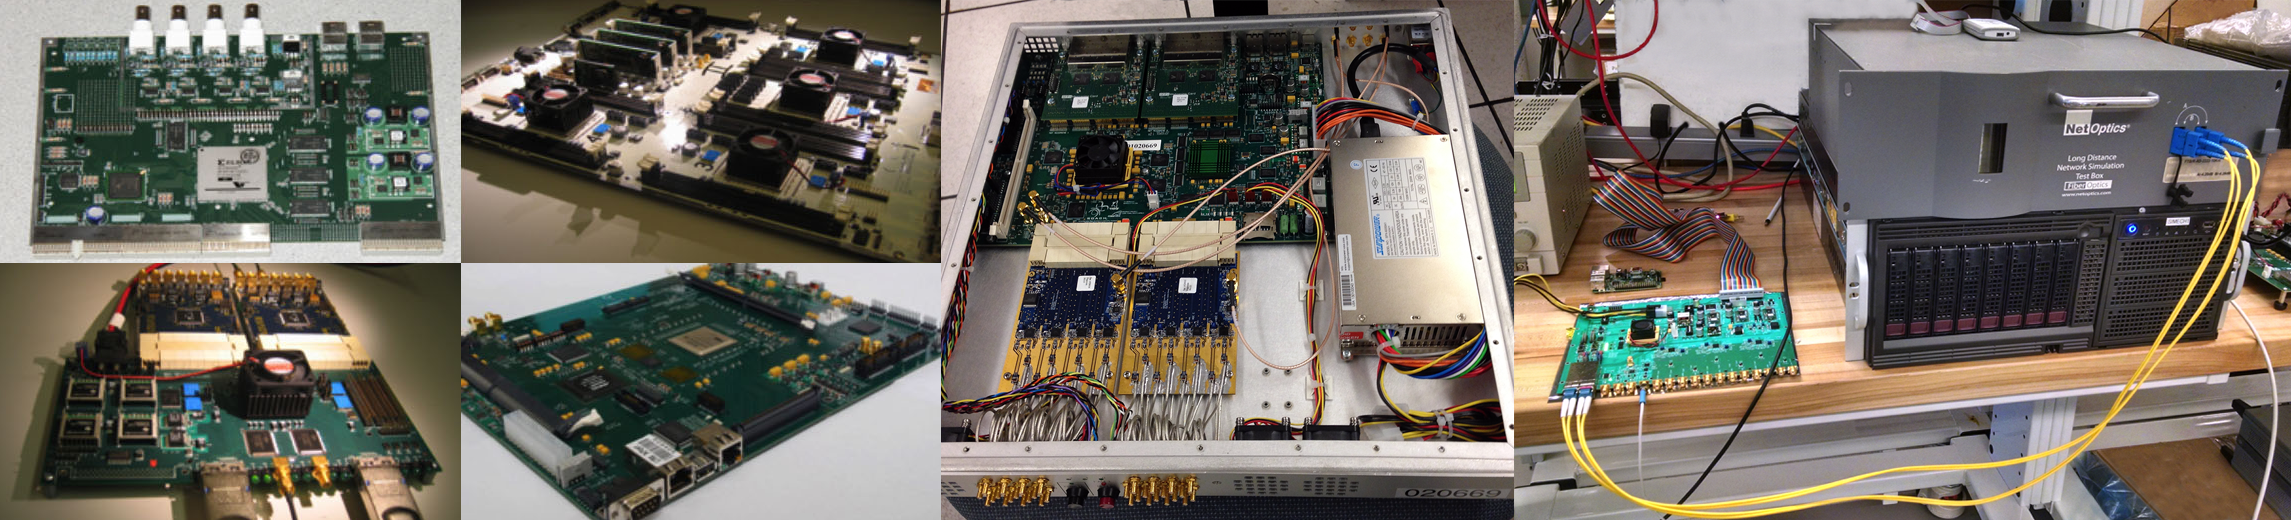
\includegraphics[width=1.0\textwidth]{plots/casper_boards.png}
%\includegraphics[height=1.7in]{plots/snap_board.png}
\caption{
Six generations of CASPER digital signal processing (left to right) culminating in the SNAP board (right, along with the long-haul fiber-link test setup), which was developed and tested under the previous HERA MSIP award.
By preserving its toolflow, signal processing libraries, and interface code between hardware generations,
CASPER combines with a scalable correlator architecture to enable the PAPER correlator to be 
easily upgraded for HERA \Mycitep{parsons_et_al2006,parsons_et_al2008}.
%
}\label{fig:hardware}
\end{figure}

{\bf Central Container}.
HERA's central container houses two significant subsystems adjacent to the array.  The first is a timing subsystem
that maintains a GPS-disciplined oscillator and distributes timing
signals (the sampling clock and 1 pulse-per-second synchronization) to the nodes.  The second
subsystem is a passive fiber optic patch panel that couples
the optical network from the nodes into the 192-filament optical fiber bundle 
that connects to the KAPB. 

{\bf Karoo Array Processing Building (KAPB)}.
The KAPB houses the switch and CPUs
that 
complete the HERA correlator system.  A fiber optic bundle enters the KAPB and patches
into local fiber optic cables. These cables terminate in optical transceivers which plug into a 240-port 10 GbE switch.
Such switches, while large, are readily available commercially today.  Also connected to
this switch are 30 servers, each hosting two dual-GPU graphics cards and two dual
10 GbE network interface cards, which implement the cross-multiplication (X-Engine) component
of the correlator during observations.  This estimate for the number of X-Engine servers
is extrapolated from current GPU servers deployed on PAPER, assuming no improvement in bus
speeds for transferring data into the GPU cores, but assuming that the computational
capacity of GPU cores doubles once according to Moore's Law prior to purchasing
these servers in year three of the project.
Output data from the correlator are written to the data storage system described
in the following section.

\subsection{Data Management}
\label{sec:data}
\noindent The HERA correlator generates $\sim4$~TB of raw data per 12-hour observing day.
HERA's data management system archives this on-site in a 1.5 PB storage array, calibrates it in real-time
on the basis of redundancy, compresses it by a factor of 20, and transfers it to our computing facility at NRAO.
This real-time pipeline, based on a similar system for PAPER, is mature, computationally manageable, and 
relatively agnostic with respect to observing parameters, making it a safe and robust first step in data processing
\citep{zheng_et_al2014,parsons_etal2014,ali_et_al2015}.
The Internet link between the Karoo and data centers in the U.S.\ has been extensively tested, with assistance from SKA-SA, TENET
(South African to London link provider) and GEANT (London to U.S.\ provider).   
Transfer speeds are sufficient for streaming compressed data to the U.S.\ via the Internet. Portable storage is also
provisioned as a fallback transfer method.

With support from this grant, NRAO hosts the archiving, indexing, and processing of HERA data products. 
Project data and public data products are served via the existing 
NRAO archive at the Domenici Science Operations Center %(DSOC) 
in Socorro, New Mexico, where it will be accessible through computing accounts and public web-based
archive searches.
NRAO also supports
an attached 30-node processing cluster 
coupled to 
scratch storage
for routine data inspection and lightweight analysis tasks.
For the bulk application of processing-intensive data pipelines to HERA data,
NRAO manages the dynamic acquisition of computing from
external HPC and cloud-computing facilities, including the Amazon spot market and XSEDE. 
Combined with legacy computing resources at UPenn and MIT, this plan leverages NRAO's
expertise in managing and acquiring computing resources while providing distributed
permanent resources for HERA's basic processing needs.


%This effort leverages existing infrastructure at NRAO, with support 
%for the expansion of the data storage and for upgrading to a 30-node computing cluster.  This cluster supports the bulk of the analysis by HERA collaborators (see \S\ref{sec:analysis}) that requires access to the full set of HERA observations.

\subsection{Analysis Pipelines} 
\label{sec:software}

\noindent HERA builds on the rich legacy of PAPER and MWA software and database systems 
developed for field operations, data analysis, and simulation.  Examples range from
the strictly versioned and unit-tested packages for field-deployed systems (e.g. the correlator, real-time processing, and
monitor/control systems) to loose collections of scripts written for exploratory analysis.
Software packages that support HERA analysis are open source, publicly 
hosted\footnote{Including \url{github.com/AaronParsons/aipy}, \url{github.com/JeffZhen/omnical}, 
\url{github.com/MiguelFMorales/FHD}, \url{github.com/MiguelFMorales/eppsilon}, \url{github.com/jpober/21cmSense},
and \url{github.com/Nithyanandan/PRISim}.}, revision controlled, and unit-tested.  
These include Omnical, a complete package for redundant baseline calibration;
Astronomical Interferometry in Python (AIPY), a set of
tools and file-format interfaces for reading visibilities, calibrating,
rephasing, imaging, and deconvolution; Fast Holographic Deconvolution
(FHD), a purpose-built tool for imaging, calibration, and foreground
forward-modeling and subtraction \citep{sullivan_et_al2012}; Precision Radio Interferometry Simulator 
(PRISim), a package for accurately simulating wide-field interferometric observations;
21cmFAST, a fast, semi-numerical 21~cm signal simulator,
and 21cmSense, a tool for forecasting power spectrum sensitivity.
Other project code is aggregated and revision
controlled in a public repository with separate sandboxes for each developer to ensure that
HERA members have up-to-date copies of all project code to facilitate sharing and debugging.
Such code includes the PAPER pipeline for foreground filtering and estimating power spectra from
visibility data,
the MWA power spectrum analysis codes---\eppsilon\ \citep{hazelton_et_al2016} and the 
empirical covariance technique of \citet{dillon_et_al2015}---as well as
machine-learning-based source finding, verification, and removal tools \citep{caroll_et_al2016,jacobs_et_al2016,beardsley_et_al2016}. 


New software development will focus on integrating and improving the MWA and PAPER power spectrum and foreground removal pipelines,
developing a monitor and control software interface and database for recording instrument metadata,
extending, with support from Scuola Normale Superiore, semi-analytic and numerical models 
of the 21~cm signal for robust parameter estimation, and developing
machine learning interpolations of simulations for joint Monte Carlo estimation of cosmological and astrophysical parameters.


\section{Schedule and Status}
\label{sec:status}

\noindent On-site construction will proceed in stages, starting from the
initial 37 elements that will be in place by project start.  These will be used
in conjunction with the thoroughly characterized extant PAPER signal path and
processing hardware for a very low risk initiation of scientific observations
from the very beginning.  Additionally, the 19 HERA elements currently in
place will also have had an extensive period of commissioning
and characterization.  As elements 38 to 128 are installed in year 1, they can
immediately be placed within the array and be used for observing.

During this period, infrastructure for the new node-based system is installed
and tested with the first elements beyond 128.  After the HERA-128 observing
season, the full array is transitioned to use HERA's new hardware infrastructure.  In this same time frame, the existing PAPER processing
container is moved to the edge of the array to house the timing sub-system
and fiber optic splice cabinet while the correlator will move to the KAPB.
Also, the data processing activity at Penn is transitioned to NRAO.
Summarizing, the hardware deployment phases are in four categories:
\begin{enumerate}
\item Element construction:  linear process (years 1, 2 \& 3)
\item Infrastructure:  (a) node power and fiber reticulation (years 1 \& 2), (b) container relocation (year 1), (c) node installation (years 2 \& 3)
\item Signal path:  convert to node-based system after 128 elements (years 2 \& 3)
\item Processing:  (a) data processor/server to NRAO (year 1), (b) X-engine \& real-time processor/storage to KAPB (year 2)
\end{enumerate}

\begin{figure}[h]
	\vspace{-7pt}
	\begin{tabular}{ll}
	\begin{minipage}{5in}
		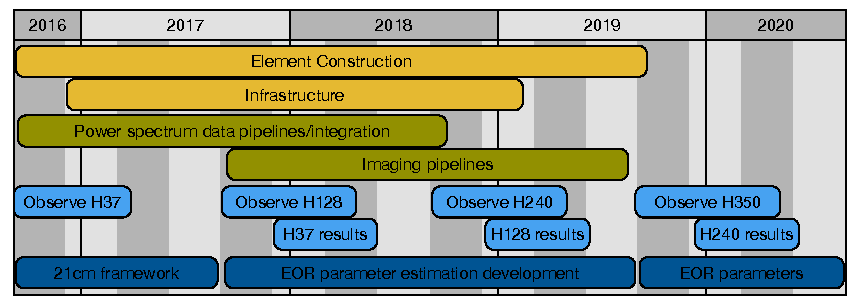
\includegraphics[width=4.9in]{plots/timeline_short.pdf}
		\end{minipage} & \hspace{-.15in}
	\begin{minipage}{1.35in}
\captionsetup{justification=raggedright,
singlelinecheck=false
}
	\caption{Timeline of HERA construction, analysis development, observation, and scientific output.}
	\label{fig:timeline}
	\end{minipage}
	\end{tabular}
	\vspace{-8pt}
\end{figure}



The optimal EoR observing window is from September to April, with power spectrum limit results appearing about one year later.  Concurrent technique development and deployment will be on-going. Additional information is in the project management plan.
\begin{itemize}[leftmargin=0.7in]
\item[Year 1:] Observe with H37.  Real-time data pipeline, delay-space power spectrum (DSPS) pipeline, FHD pipeline.  21\,cm framework for incorporating with other probes. Construct H128.
\item[Year 2:] Observe with H128.  Real-time calibration pipeline.  DSPS/FHD/global sky model integration. Snapshot imaging pipeline.  EoR parameter estimation development.  H37 results.  Construct H240.  {\em Data products:  power spectrum, Stokes I maps.}
\item[Year 3:] Observe with H240.  Foreground-filtered imaging pipeline.  EoR parameter estimation development.   H128 results. Construct H350.  {\em Data products:  power spectrum, Stokes IQUV maps, foreground image cube.}
\item[Year 4:] Observe with H350.  EoR parameter estimates.  H240 results.  {\em Data products:  power spectrum, global sky model IQUV, snapshots, foreground-filtered image cube.}
%\item[Year 5:] Observe with H350.  H350 results.  {\em Data products:  power spectrum, global sky model IQUV, snapshots, foreground-filtered image cube.}
\end{itemize}

\section{Conclusion}
\label{sec:conclusion}

\noindent With first-generation instruments, the HERA team has led a revolution in our understanding of how to best perform 21\,cm cosmology measurements.
In the past three years, we have developed the EoR window paradigm for isolating foreground systematics, implemented novel
calibration and power spectrum analysis pipelines, made precision measurements of astrophysical foregrounds, and published deep power 
spectrum limits that constrain heating in the early universe.  HERA's design, now validated in the field with MSIP seed funding, 
is the result of these advances.


HERA is ``the right instrument at the right time.'' With first generation experiments approaching the limits of their sensitivity, it is now critical to build upon our new knowledge and experience to advance beyond them. HERA's large collecting area and optimized design enable precise constraints of EoR astrophysics and a broad range of high-impact secondary science, all before SKA-low becomes operational.
With CHAMP, HERA expands CAMPARE's proven methods and recruitment network to bring more students from underrepresented groups into cutting-edge astronomy research and support them with year-round mentoring.
By bringing the U.S.\ teams from PAPER, the MWA, MITEoR, and EDGES together with strategic international partners,
the HERA collaboration has consolidated theoretical and experimental leadership in the field, 
and is equipped to deliver the proposed science. By building HERA, we can provide the community with unprecedented insights into this key new area of cosmology.


\clearpage
\setcounter{page}{1}
\thispagestyle{empty}
%\bibliographystyle{apj}
%\bibliographystyle{hapj}
\nocite{Beardsley:thesis}
\nocite{kolopanis_et_al2016}
\bibliographystyle{jponew}
%\bibliographystyle{unsrt}
{\small \bibliography{biblio}}


\end{document}

